% *****************************************************************************
%
% Author: Léonard Binet
%
% Professional thesis report.
%
% *****************************************************************************


\documentclass[a4paper, 12pt]{report}


\usepackage{geometry}
\usepackage[english]{babel}
\usepackage[utf8]{inputenc}
\usepackage[T1]{fontenc}
%\usepackage{graphicx}
%\usepackage[pdftex]{graphicx}
\usepackage{setspace}
\usepackage[pdftex]{hyperref}
\usepackage{amsmath,amsthm,amsfonts,amssymb}
\usepackage[T1]{fontenc}
\usepackage{multirow}
\usepackage{svg}
\usepackage{float}
\usepackage{textcomp}
\usepackage{fullpage}
\usepackage{fancyvrb}
\usepackage{fancyhdr}
\usepackage{lmodern}
\usepackage{sistyle}
% \usepackage{color}
\usepackage{xcolor}
\usepackage{float}
\usepackage{wrapfig}
\usepackage[justification=centering, font={small}]{caption}
\usepackage{verbdef}
\usepackage{dsfont}
\usepackage[normalem]{ulem}
\usepackage{amssymb} % for mathbb
\usepackage{outlines}

% for diagrams
\usepackage{tikz}
\usetikzlibrary{shapes,arrows, positioning}

% force footnotes to be on the bottom
\usepackage[bottom]{footmisc}

% for tables
\usepackage{booktabs}
\usepackage{tabularx,ragged2e}
\newcolumntype{L}{>{\arraybackslash}X}

% for pseudocode
\usepackage{algorithm}
\usepackage{algorithmic}
% \usepackage[noend]{algpseudocode}

% bigger operators
\usepackage{relsize}

% neural figures
\usepackage{tikz}
\def\layersep{2.5cm}


% for cases
\makeatletter
\renewcommand{\env@cases}[1][@{}l@{\quad}l@{}]{%
  \let\@ifnextchar\new@ifnextchar
  \left\lbrace
  \def\arraystretch{1.2}%
  \array{#1}%
}
\makeatother

% Remove indent of 2nd paragraph in sections, subsections, etc.
% Uncomment to enable
\setlength{\parindent}{0pt}

\newcommand\Framing[1]
  { \hspace{10mm}
     \framebox{#1}\hspace{10mm}}

% nested bullet lists
\renewcommand{\labelitemii}{$\star$}

% For json
\usepackage{bera}% optional: just to have a nice mono-spaced font
\usepackage{listingsutf8}
\usepackage{xcolor}

\colorlet{punct}{red!60!black}
\definecolor{background}{HTML}{EEEEEE}
\definecolor{delim}{RGB}{20,105,176}
\colorlet{numb}{magenta!60!black}

\lstdefinelanguage{json}{
    basicstyle=\normalfont\ttfamily,
    numbersep=8pt,
    showstringspaces=false,
    breaklines=true,
    frame=lines,
    backgroundcolor=\color{background},
    extendedchars=false,
    escapeinside={\%*}{*)},
    breakatwhitespace=true,
    inputencoding=utf8,
    literate=
     *{:}{{{\color{punct}{:}}}}{1}
      {,}{{{\color{punct}{,}}}}{1}
      {\{}{{{\color{delim}{\{}}}}{1}
      {\}}{{{\color{delim}{\}}}}}{1}
      {[}{{{\color{delim}{[}}}}{1}
      {]}{{{\color{delim}{]}}}}{1},
}

% -----------------------------------------------------------------
%                              Tools
% -----------------------------------------------------------------

% Adding source to figures
\newcommand*{\captionsource}[2]{%
  \caption[{#1}]{%
    #1%
    \\\hspace{\linewidth}%
    \textbf{Source:} #2%
  }%
}
% Format multiline text in subscripts
\newcommand\multiLine[1]{\text{\scriptsize\tabular[t]{@{}l@{}}#1\endtabular}}

\newcommand{\reporttitle}{Product data-quality improvement through attribute prediction}
\newcommand{\reportauthor}{} % Auteur
\newcommand{\reportsubject}{Professional Thesis} % Sujet
\newcommand{\HRule}{\rule{\linewidth}{0.5mm}}
\setlength{\parskip}{1ex} % Espace entre les paragraphes

% indent a paragraph
\newenvironment{myindentpar}[1]%
 {\begin{list}{}%
         {\setlength{\leftmargin}{#1}}%
         \item[]%
 }
 {\end{list}}

% -----------------------------------------------------------------

\geometry{top=2.5cm,left=2.6cm,right=2.6cm,bottom=2.5cm,headsep=1cm}
\hypersetup{pdfborder={0 0 0},
colorlinks,urlcolor=blue,linkcolor=blue,citecolor=blue,filecolor=blue,
pdftitle=
}


\begin{document}

\pagestyle{fancy}
\fancyhead[C]{Léonard\, Binet}
\fancyhead[R]{Telecom ParisTech}
\fancyhead[L]{Alkemics}

\cfoot{\thepage}
\setlength\headheight{15pt}

% Inspiré de http://en.wikibooks.org/wiki/LaTeX/Title_Creation

\begin{titlepage}

\begin{center}

\begin{center}
    
\includegraphics[height=3cm]{images/logo-telecom-paristech.png}
    \hspace{\stretch{1}}
    
\includegraphics[width=6cm]{images/Logo-Alkemics.png}
\end{center}

\vspace{160pt}

\textsc{\Large \reportsubject}\\[0.5cm]
\HRule \\[0.4cm]
{\huge \bfseries \reporttitle}\\[0.4cm]
\HRule \\[1.5cm]

\vspace{50pt}

 \large{\textbf{Léonard Binet} \\ Telecom ParisTech \\ Post-Master's Degree \\ BGD \\ \vspace{0.25cm} - \vspace{0.25cm} \\
  Company supervisor: Pierre Arbelet \\ Academic supervisor: Slim Essid}

\vfill

{\large January 01, 2018}

\end{center}

\end{titlepage}

\begin{abstract}

Confronted with challenges concerning product data quality, Alkemics decided to explore new ways to provide value proposition to its clients.

This paper aims at explaining how we tackled data-quality challenges at Alkemics, with the use of some machine learning algorithms.
But rather than solely describing models and algorithms, a focus is put on implementation and business added value. 


\end{abstract}


\cleardoublepage   % Dans le cas du recto verso, ajoute une page blanche si besoin
\tableofcontents % Table des matières
\sloppy            % Justification moins stricte : des mots ne dépasseront pas des paragraphes

\cleardoublepage
\chapter{Introduction}

Alkemics is a start-up that was founded in 2011. Back then, they created e-merchandising tools to improve user experience on e-commerce websites. It then evolved to become a platform that enables the FMCG (Fast-Moving Consumer Goods) ecosystem to share all their data, from product to transactional information, in order to improve pricing, supply, marketing.

Alkemics develops products that enable collaboration between Brands and Retailers, and tackle the challenges of omni-channel commerce and smart customer interaction.

\section{Alkemics}

\begin{figure}[H]
\centering
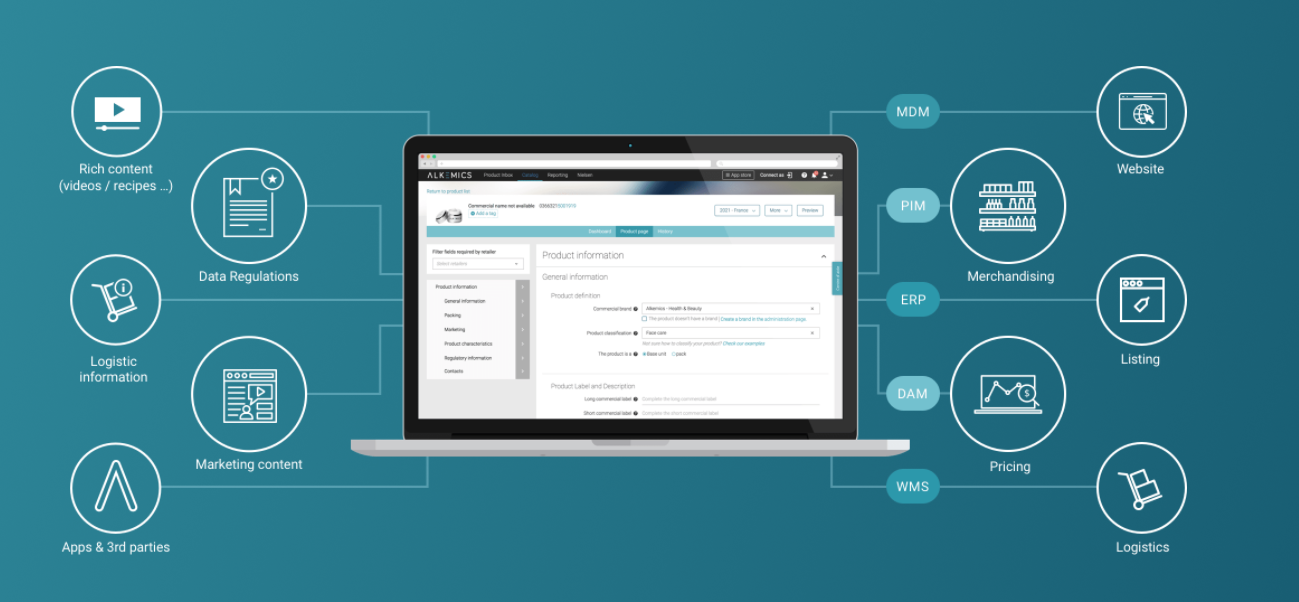
\includegraphics[scale=0.30]{./images/alkemics_website_global.png}
\caption{Alkemics}
\end{figure}

\subsection{Product Data Empowerment}

Because of increasing regulations, new customer demands, omni-channel communications, there is a growing need for richer and more exhaustive product information as well as an exponentially growing number of products. Some products change more than 10 times per year (promotion, seasonality, new recipes, new packagings...), and overall, 40\% of products are renewed every year.

This cascades in a series of problems that handicap manufacturers, retailers and consumers: logistics struggle to maintain stock, accounting systems fail to track how different products are actually the same consumption unit, pricing teams struggle to maintain price coherency in this dynamic environment, marketing teams are inefficient to share richer and richer content about the product, BI teams feel that the consumption of the consumer are changing while they actually don't.

This problem is called product chaining. It describes the ability to connect products that share a given set of attributes in order to understand how they relate.

To overcome these problems, Alkemics built a product taxonomy reinforced by an ontology. PDE \footnote{Product Data Empowerment} team is fully dedicated to enhance the classification task to automatically classify the category of products, as well as the brand and other attributes such as the packaging or the price range. The classification task mainly uses Natural Language Processing techniques and distances in semantic spaces. PDE is also in charge of the management of the product data model.


\subsection{Product Stream}

Product Stream is a web application that enables:
\\

\textbf{Makers} to:
    \begin{itemize}
    \item Collect product information from all the stakeholders of the organization: the \textit{supply team} who knows the size and weight of the product, the \textit{marketing team} who owns the pictures, videos as well as the brand content, the \textit{quality team} who masters the composition, nutritional values, etc.
    \item Store product information in a centralized way, so everyone in the organization can have access to it (DAM \footnote{Digital Asset Management}).
    \item Distribute product information so every partner has the same up-to-date information. This includes retailers, but also marketing agencies, trade marketing agencies, ... (EDI \footnote{Electronic Data Interchange} / PIM \footnote{Product information management})
    \item Collaborate with 3rd parties to collect user reviews,  receive data quality reports,  print coupons, use buy-it-now solutions.
    \end{itemize}

\textbf{Retailers} to:
    \begin{itemize}
    \item Have access to best-in-class product information to power their tools and feed their digital supports (EDI)
    \item Collaborate with manufacturers to reference new products \& innovations, run call-for-proposals for promotional formats, etc…
    \item Connect products that share a given set of attributes in order to understand how they relate (Product Chaining).
    \end{itemize}

\subsection{The technological stack}

\textbf{Micro-services architecture}
The stack in Alkemics is composed of set of dozens of micro services communicating with synchronous calls (HTTPS) and both synchronous and asynchronous messaging (TCP enabled by Rabbit MQ).
Each service has a domain specific task: data ingestion, data classification, APIs for merchandising, etc. A subset of the services are exposed to third parties and clients.

\textbf{User interface}
User Interface dashboards also call the APIs to make functionalities available to the users (makers and retailers) trough a web browser.
The front part of the website is implemented with React framework.

\textbf{APIs and SDKs}
A set of SDKs are also provided to retailers to allow them to use merchandising functionalities directly embedded in their websites.

\textbf{Storage vs indexation}
All Alkemics crucial data is stored in relational databases (MySQL). Yet if relationnal databases provide very useful functionalities to guaranty integrity of data, its indexing capabilities remain quite poor in comparison to non-relational databases.

That's we also create ElasticSearch indexes, containing data that is already stored in relational databases, but indexed in a format allowing quick and performant queries.


\section{Professional thesis objective}

This professional thesis aims at implementing machine learning techniques to improve products data quality.

\cleardoublepage
\chapter{Data quality challenge}

This chapter details one of the main challenges Alkemics faces, and how we tackled it. 
After presenting what is data-quality and why it matters, we will present how we built a suggestion workflow that helps our users to detect errors, and provides potential corrections. Finally we will detail what tools we built to monitor and control quality.

The detail of machine learning algorithms used to provide predictions will be detailed in next chapter.

\section{Stakes}

Reliable, up-to-date, accessible, tracable, product data is one of the core value proposition of Alkemics services for retailers.

To provide this service, Alkemics teams have put a lot of effort in building:

\begin{itemize}
	\item bridges between data-models: Mondelez data-model is not the same as Pepsi, or Auchan's one. Alkemics data-model aims at generalizing all others and have the ability to translate any product data in other data-models.
	\item bridge between data-stores: APIs and interfaces to easily import or export data in several formats.
	\item bridges between people: ability to communicate easily about products through the platform
\end{itemize} 

Ultimately, data is owned and provided by manufacturers, and then shared with retailers.

\subsection{What is data-quality}

\begin{figure}[H]
\centering
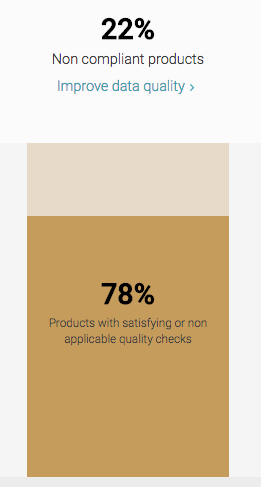
\includegraphics[scale=0.50]{./images/data-quality/data-quality-2.png}
\caption{Example of data-quality measure.}
\end{figure}

Data quality can be evaluated through:
\begin{itemize}
\item completeness: the product page has sufficient details about the product.
	\begin{itemize}
		\item regulatory fields: for instance if your product contains alcohol you must provide the alcohol concentration.
		\item retailer specific fields: some retailer set their own requirements to sell on their platforms
	\end{itemize}
\item accuracy: the provided data is accurate, there is no error.
\end{itemize}

\begin{figure}[H]
\centering
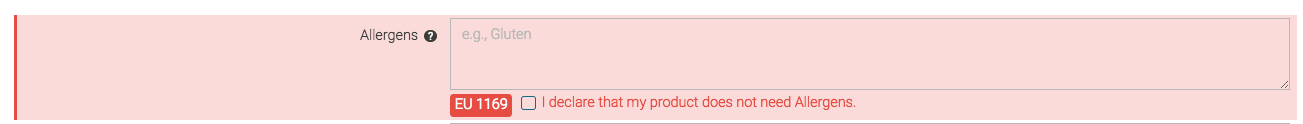
\includegraphics[scale=0.45]{./images/data-quality/data-quality.png}
\caption{Example of a product that doesn't specify required fields.}
\end{figure}

\subsection{Why it matters}

\textbf{Data quality is a major issue to retailers}

\begin{itemize}
\item Regulatory: internet retailers have the obligation to provide some specific informations on the products. If they don't they can be heavily fined. Fields as 
\item Marketing: display detailed information about products to customers. Would you buy products with no description?
\item Search: to correctly index products you need data, for instance how will your customer find strawberry icecream is flavors fields are not well filled. Well indexed products is key to performant search engine on web plateforms.
\item Logistics: weight, size, number of units etc. These fields allow retailers to correctly handle logistics.
\item Competition: the rise of Amazon is a direct threat to all retailers. One of Amazon's advantages is its huge ability to handle data-flows.
\end{itemize}


\subsection{Why is the data of poor quality}

Some of the reasons are:

\begin{itemize}
\item many actors have to communicate: more than 50 thousands of manufacturers have to interact with dozens of retailers. Each manufacturer has to send its data to each retailer sending its products. This represents hundreds of thousands of connections.
\item no fully accepted data-model standard. Even though GDSN standard is dominant, not all companies are compliant with it.
\item actors interested in data-quality (primarly retailers), rely on actors for which it is less crucial (makers)
\item products data identification numbers (EAN) frequently change
\end{itemize}

\subsection{What can we do about data-quality}

Given a product, we want to predict several of its attributes given some basic fields that are nearly always filled.
The predicted fields for now are:
\begin{itemize}
	\item hazard pictograms (inflammable, corrosive etc ...)
	\item labels (organic, made in France, eco-packaging etc...)
	\item kind: category in Alkemics data-model (Processed meat, Cereal, baked product etc...)
	\item allergens (walnut, lactose, sulfite etc ...)
	\item flavors
\end{itemize}

\begin{figure}[H]
\centering
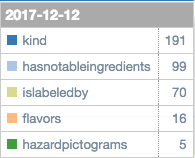
\includegraphics[scale=0.55]{./images/workflow/predicted_fields.png}
\caption{Number of distinct classes per predicted attribute.}
\end{figure}

After these predictions are made, we want to evaluate it against products attributes to warn the manufacturers if we think that some of its data is incomplete or innacurate.

\subsection{What are our constraints}
\begin{itemize}
\item we cannot unilaterally change manufacturers data: they own their data
\item we must garanty a high degree of confidence on suggestions we make, especially at the begining, otherwise manufacturers won't trust and use our suggestions
\item predictions must be made regularly (product data continuously evolve)
\item predictions must adapt to data-model changes
\item our predictive models hade to perform well on datasets of poor data-quality (some fields are nearly never filled)
\item we must be able to monitor closely how well our models perform, and how well perceived are our suggestions 
\end{itemize}


\pagebreak
\section{Suggestion Workflow to improve data-quality}


This part aims at presenting the workflow we use to provide attribute suggestions on product-pages to our users.

During the creation of this workflow, we sticked to some best practices for machine learning engineering, among those listed in a Google paper \cite{RulesMLGoogle} we can cite:
\begin{itemize}
	\item keep the model simple and get the infrastructure right (rule 4)
	\item test the infrastructure independently from the machine learning (rule 5)
	\item starting with an interpretable model makes debugging easier (rule 14)
\end{itemize}

\begin{figure}[H]
\centering
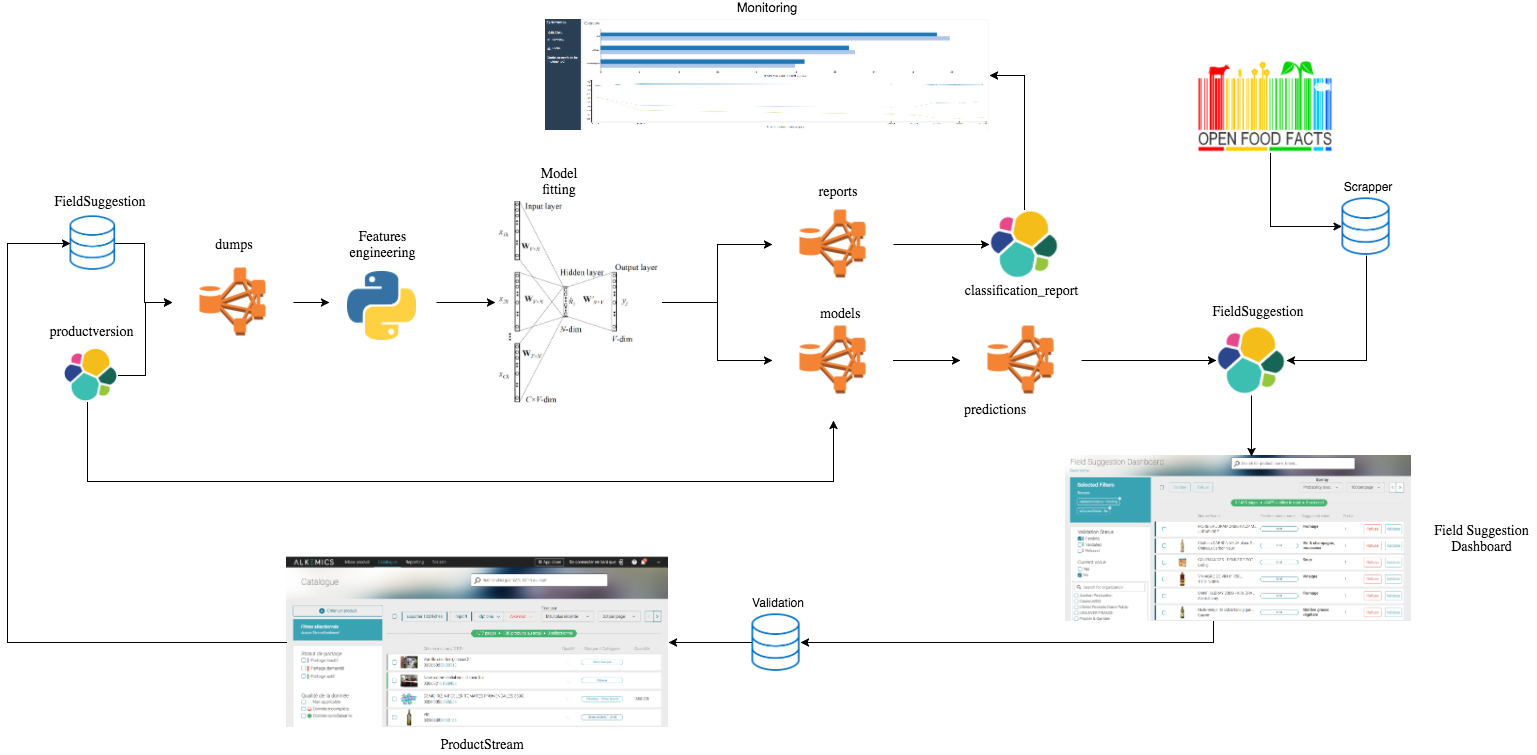
\includegraphics[scale=0.30]{./images/workflow/fieldsuggestion-workflow.png}
\caption{Suggestion workflow overview.}
\end{figure}

\subsubsection{Workflow steps}
\begin{enumerate}
	\item extraction of some attributes (name, description, composition) from products
	\item feature engineering (NLP preprocessing)
	\item training on labeled products (fasttext model) and report
	\item prediction (on all products)
	\item indexation as suggestion
	\begin{itemize}
		\item from machine learning suggestions
		\item from scrapped websites (major one: OpenFoodFacts)
	\end{itemize}
	\item suggestion validation by Alkemics
	\item display of validated suggestions to users in product pages
	\item suggestion acceptation by users
\end{enumerate}


% For product 1198365 / 07622300788063: https://stream.alkemics.com/#/catalog/07622300788063


\subsection{Feature and labels extraction}

In our data-model, a product can consist of more than one hundred of fields, yet only some of them can be sufficient.
The idea is to find a compromise between gathering enough information from products (-> more fields), but on fields with sufficient completion (-> less fields). For now we chose to only use textual data, and let aside pictures (we might use them in the future).

Let's take a cereal bar of brand Grany:
\begin{figure}[H]
\centering

\includegraphics[scale=0.50]{./images/sample/grany_picture.png}
\caption{Product for which we will try to improve data-quality.}
\end{figure}

Here are the extracted attributes that will be processed to provide our features.

\begin{minted}[breaklines, fontsize=\small]{json}
{
    "brand": "Grany",
    "namePublicLong": "Grany Coeur Fondant Gout Chocolat Noisettes 120g",
    "nameLegal": "BARRE CEREALIERE FOURREE AU CHOCOLAT ET A LA NOISETTE.",
    "composition": "Ingrédients: Céréales 31,5% (farine de RIZ 9,1%, farine de BLÉ 5,6%, grains de maïs 4,7%, flocons de BLÉ 4,5%, flocons d'AVOINE 4,5%, flocons d'ORGE 2,5%, farine de BLÉ malté 0,6%), sirop de glucose-fructose, sucre, huile de coprah, LAIT écrémé en poudre, huile de palme, chocolat 5% (sucre, pâte de cacao), pâte de NOISETTES 5%, cacao maigre en poudre, humectant (glycérol), sel, gluten (de BLÉ), dextrose, émulsifiant (lécithine de tournesol), malt d'ORGE, arôme (NOISETTES), ARACHIDE. PEUT CONTENIR SOJA, AUTRES FRUITS À COQUE.",
    "description": "Grany au cœur Chocolat au Lait et aux Noisettes, le plaisir brut des céréales associées au fondant du chocolat au lait !",
    "advices": "",
    "healthAllegations": ""
}
\end{minted}

\subsection{Feature engineering}

Transforming these features in a relevant input format for our models. 
The models we use will be detailed in next chapter. Theses models accept similar input as famous NLP models such skip-gram or c-bow.

This is classic NLP preprocessing.

\begin{enumerate}
	\item concatenated fields as string
	\item normalize text (encoding -> ascii)
	\item tokenize
	\item for each token:
	\begin{itemize}
		\item lower
		\item remove eventual html tags
		\item filter stopwords and punctuation
		\item remove digits
		\item stem (we use NLTK package \cite{NLTK})
	\end{itemize}
	\item concatenate tokens
\end{enumerate}

Our previous object is now a list of preprocessed tokens that take the following form.

\begin{minted}[breaklines, fontsize=\small]{json}
"grany cur chocolat lait noiset plais brut cereal associe fond chocolat lait grany barr cerealier fourre chocolat noiset grany coeur fond gout chocolat noiset ingredient cereal farin riz farin ble grain flocon ble flocon avoin flocon orge farin ble malt sirop glucos fructos sucr huil coprah lait ecrem poudr huil palm chocolat sucr pat cacao pat noiset cacao maigr poudr humect glycerol sel gluten ble dextros emulsifi lecithin tournesol malt orge arom noiset arachid conten soj autr fruit coqu"
\end{minted}

\subsection{Training stage}

Training stage includes:
\begin{enumerate}
	\item labeled-set preprocessing: remove blacklisted labels, filter classes without enough occurences (we want our model to learn only labels we want to display).
	\item split training/testing sets:
	\item fit models on training set, predict on testing set
	\item compute performance and monitoring reports separatly on both train-set and test-set
	\item compute global/local precision curves
	\item save model for further use
	\item index reports for monitoring
\end{enumerate}

Labeled-set preprocessing is not the same in the case we consider multiclass or multilabel classification.
\begin{itemize}
	\item in multiclass case: every sample has one and only one label
	\item in multilabel case: a sample can be considered even though it has no label
\end{itemize}

\subsection{Predict stage}
Predict stage includes: 
\begin{itemize}
	\item extracting all product features (label AND non-labeled)
	\item compute prediction scores
	\item enrich prediction with recall/precision estimations based on prediction score and local precision/recall curves computed during training-stage
	\item save all predictions with scores > 0.05
\end{itemize}

\subsection{Machine learning suggestion indexation with scrapped information}

Suggestions from machine learning, are merged with suggestions issued from web-scrapping.
Those suggestions are indexed together to provide a global score (number of concordant sources) to suggestions.

Here is an example of a suggestion document that will be indexed in ElasticSearch. Its structure will allow us to perform complex queries and provide a validation dashboard with many functionalities.
\begin{minted}[breaklines, fontsize=\small]{json}
{
    "_type": "fieldsuggestion",
    "extended_attributes": {
        "precision_group": 0.91489,
        "features": "grany cur chocolat lait noiset plais brut cereal...",
        "probability": 0.87393,
        "recall_group": 0.55128
    },
    "field": {
        "status": 0,
        "fieldmetadata_name": "hasnotableingredients",
        "fieldmetadata_id": 107,
        "is_current_value": 0,
        "field_id": 59,
        "field_name": "arachide"
    },
    "id": "1198365_107_59",
    "metadata": {
        "global_score": 4,
        "product_id": 142292,
        "media": "https://smedia.alkemics.com/product/142292/...",
        "brand": "Grany",
        "contentowner": {
            "id": 356,
            "name": "Mondelez International"
        },
        "sources": [
            "openfoodfacts",
            "ml"
        ],
        "gtin": "07622300788063",
        "productversion_id": 1198365,
        "name": "Grany Coeur Fondant Gout Chocolat Noisettes 120g"
    }
}
\end{minted}


\subsection{Validation (or refusal) from Alkemics}
Since we must reach a high degree of confidence in our predictions, and since we do not yet have history about how well we perform, each suggestion is manually validated. 


For all predictions that are not values already stored in products' data (if the prediction match an already existing product data, everything's fine and we don't need to change its value), we will validate or refuse the suggestion.

A part of this task is semi-automated: for instance, suggestions issued from both scrapping and machine learning, with an estimated precision of 90\% are batch validated.

\begin{figure}[H]
\centering
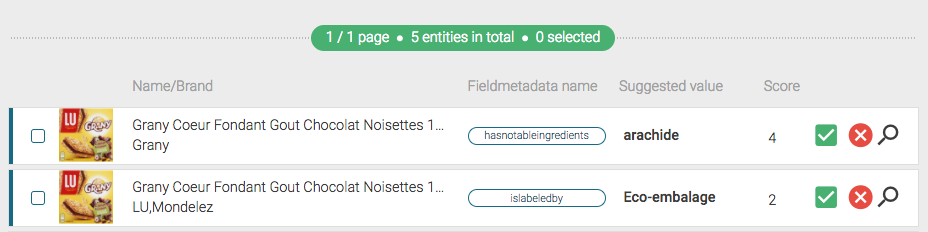
\includegraphics[scale=0.50]{./images/workflow/validation-suggestion.png}
\caption{Suggestion validation by Alkemics.}
\end{figure}


\subsection{Suggestion display to users in product pages, and acceptation (or dismissal) from manufacturer}

Now that the suggestion is validated, we notify the manufacturer in charge of this product, and include a control in his product page allowing him to easily accept of dismiss the suggestion.

\begin{figure}[H]
\centering
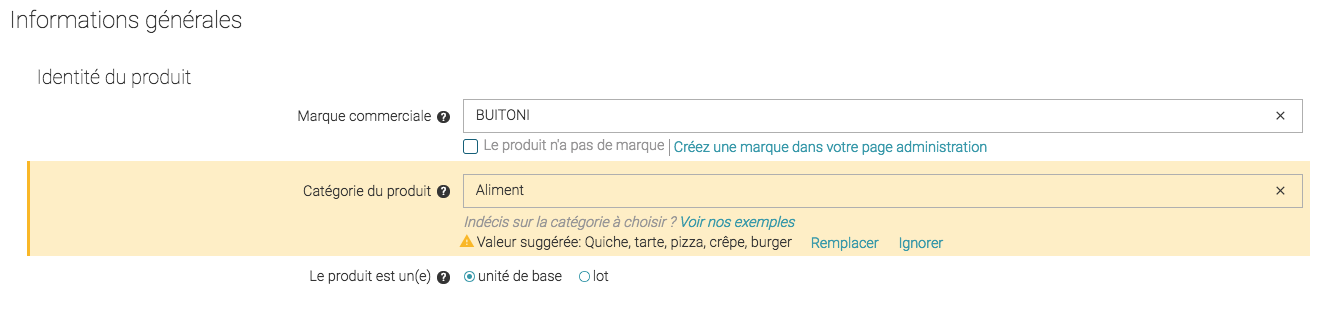
\includegraphics[scale=0.35]{./images/workflow/stream-suggestion-3.png}
\caption{Suggestion acceptation by user.}
\end{figure}

In case of acceptation, the product's data is changed in Alkemics product database. Else, in case of dismissal, we store the fact that the suggestion is 'wrong' so we don't notify the manufacturer if we repredict the same value the day after.


\pagebreak
\section{Regular maintenance and improvement tasks}

Once the workflow is deployed there are several day-to-day tasks to perform. This include monitoring the workflow to detect eventual anomalies, validating suggestions so that they are sent to users, and manually bootstrapping some classes for which our models don't perform well.

\subsection{Monitoring}

Given the complexity of the workflow, and quality expected by clients, we have to closely monitor some metrics:
\begin{itemize}
	\item did the workflow worked, if not where did it fail
	\item is there an evolution of classes distribution
	\item how our scores behave at training stage
	\item whether our predictions get rejected at validation stage
	\item do our validated suggestion get dismissed by user at acceptation stage
\end{itemize}

\subsubsection{Check workflow completion}
Our workflow consists of lots of interdependent tasks. Some of them have to be completed in a precise order. Some can be parallelized, some not. To ensure that our workflow runs as expected we use a workflow management tool: Luigi.

By defining each task dependencies (a task can depend on multiple other tasks), Luigi will draw an acyclic directed dependency graph.

Luigi library comes with a useful web interface, showing wich tasks are pending/runing/completed or have failed:
\begin{figure}[H]
\centering
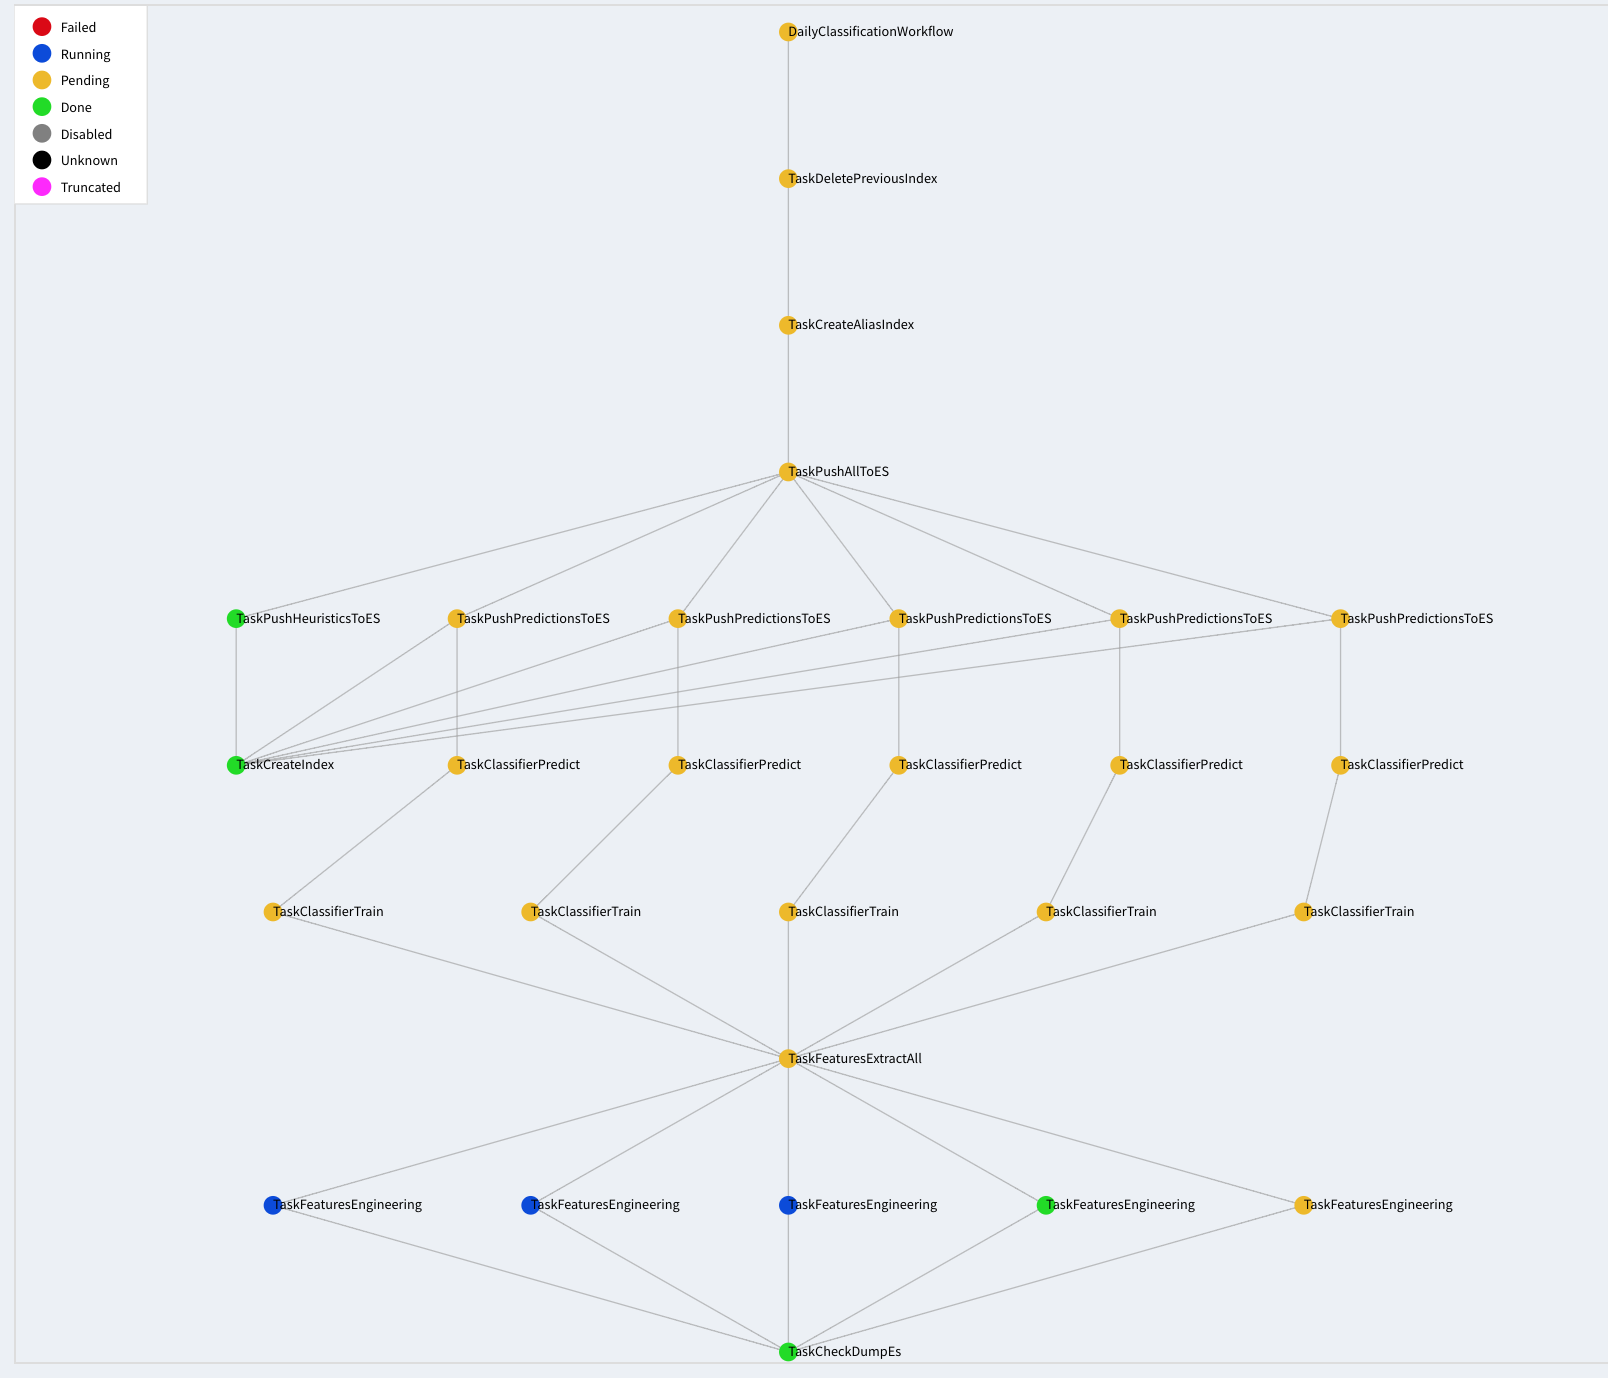
\includegraphics[scale=0.50]{./images/monitoring/luigi-graph-3.png}
\caption{Classification workflow dependency graph.}
\end{figure}

\subsubsection{See and understand scores evolution}
Knowing how our models perform is crucial to know how confident we can be into our models.

To do so I built a monitoring interface drawing the scores evolution for different fields we try to enrich.
\begin{figure}[H]
\centering
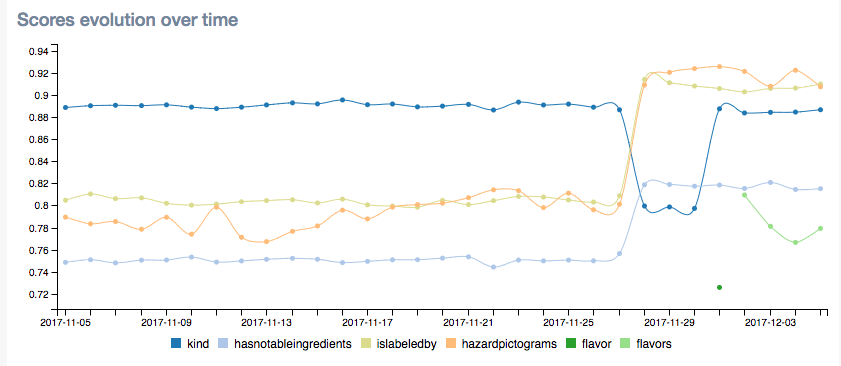
\includegraphics[scale=0.50]{./images/monitoring/global-scores-evolution-2.png}
\caption{Classification micro-average global scores evolution.}
\end{figure}

Among the different reasons why our models scores can evolve, one is the change of classes distribution, so some graphs can help check if something is wrong: in this case, the following graph helped us find why a field predictions dropped: some wrongly labeled data was introduced.

\begin{figure}[H]
\centering
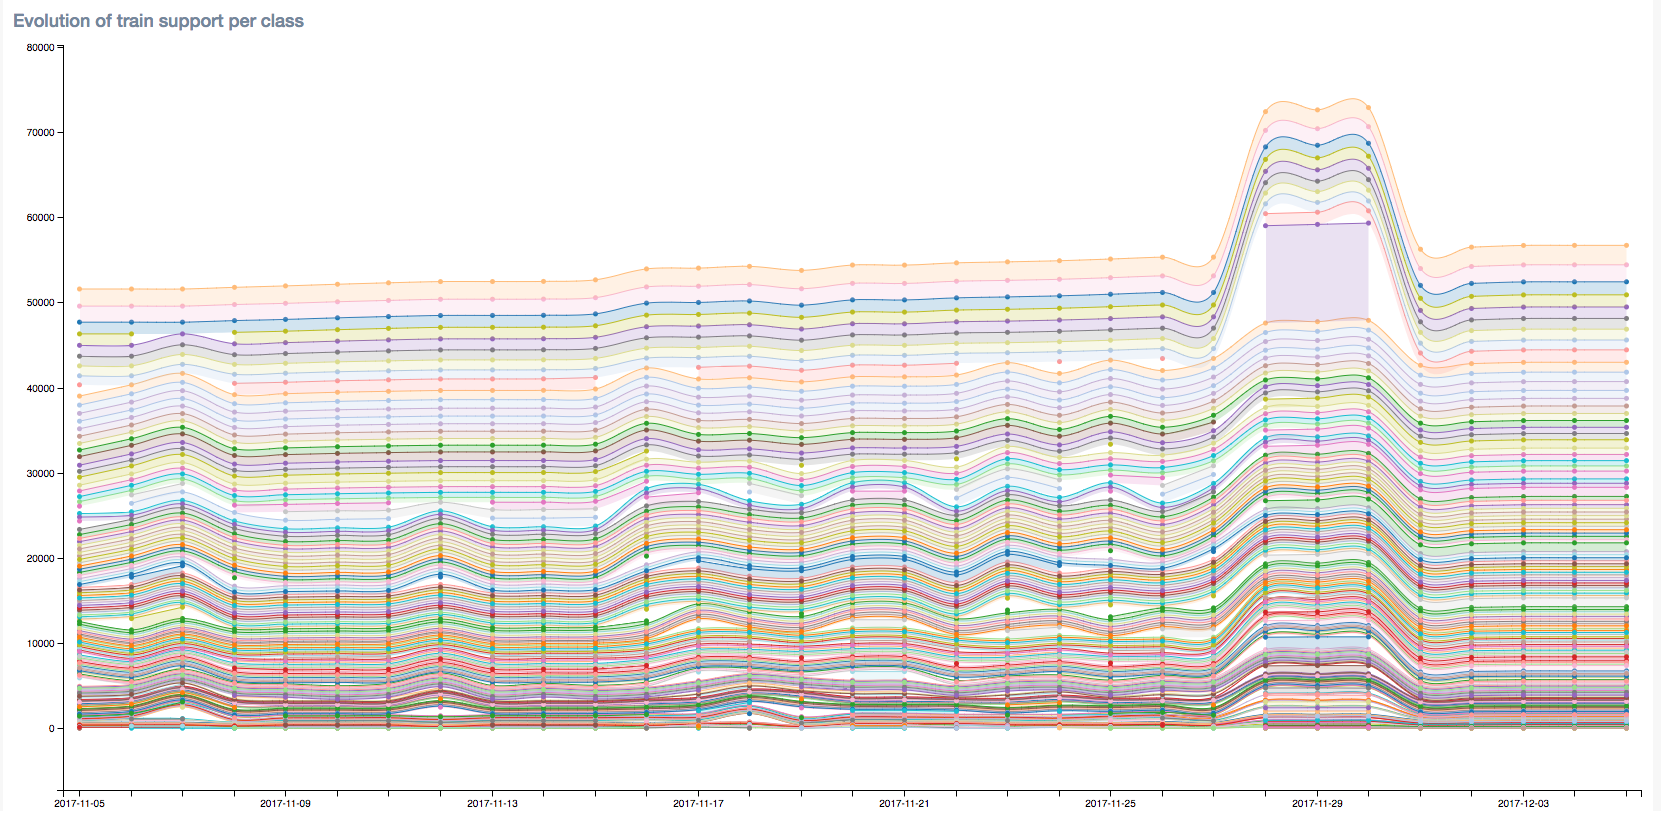
\includegraphics[scale=0.30]{./images/monitoring/local-classes-evolution.png}
\caption{Local classes distribution evolution. We can detect the creation of an invalid class that led to dropping scores.}
\end{figure}


\subsubsection{Check validation / Acceptation rates}

In machine learning, the more frequent way to estimate a model performance is to predict on a test-set and compare predictions to true labels of the test-set.

In our case, we can also check the validation/refusal ratio at validation stage:

\begin{figure}[H]
\centering
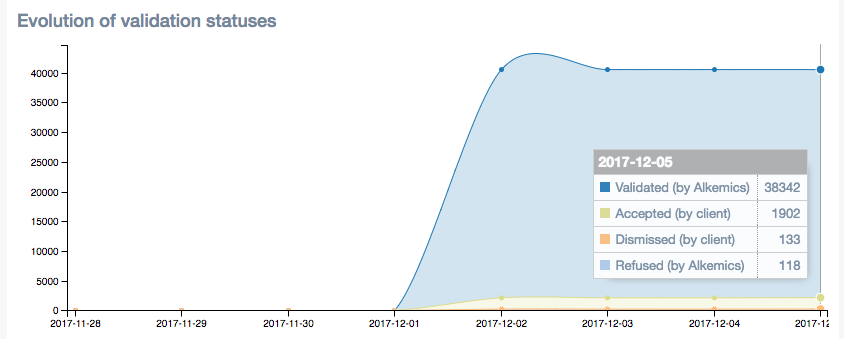
\includegraphics[scale=0.50]{./images/monitoring/validation-acceptation-monitoring.png}
\caption{Validation/Acceptation rates.}
\end{figure}

\subsubsection{Evaluate business impact}

Number of views, and acceptation rates.

\subsection{Deliver validated suggestions}

By a mix of automation and manual validation.
A big effort has been made to build an internal suggestion validation dashboard. 

\begin{figure}[H]
\centering
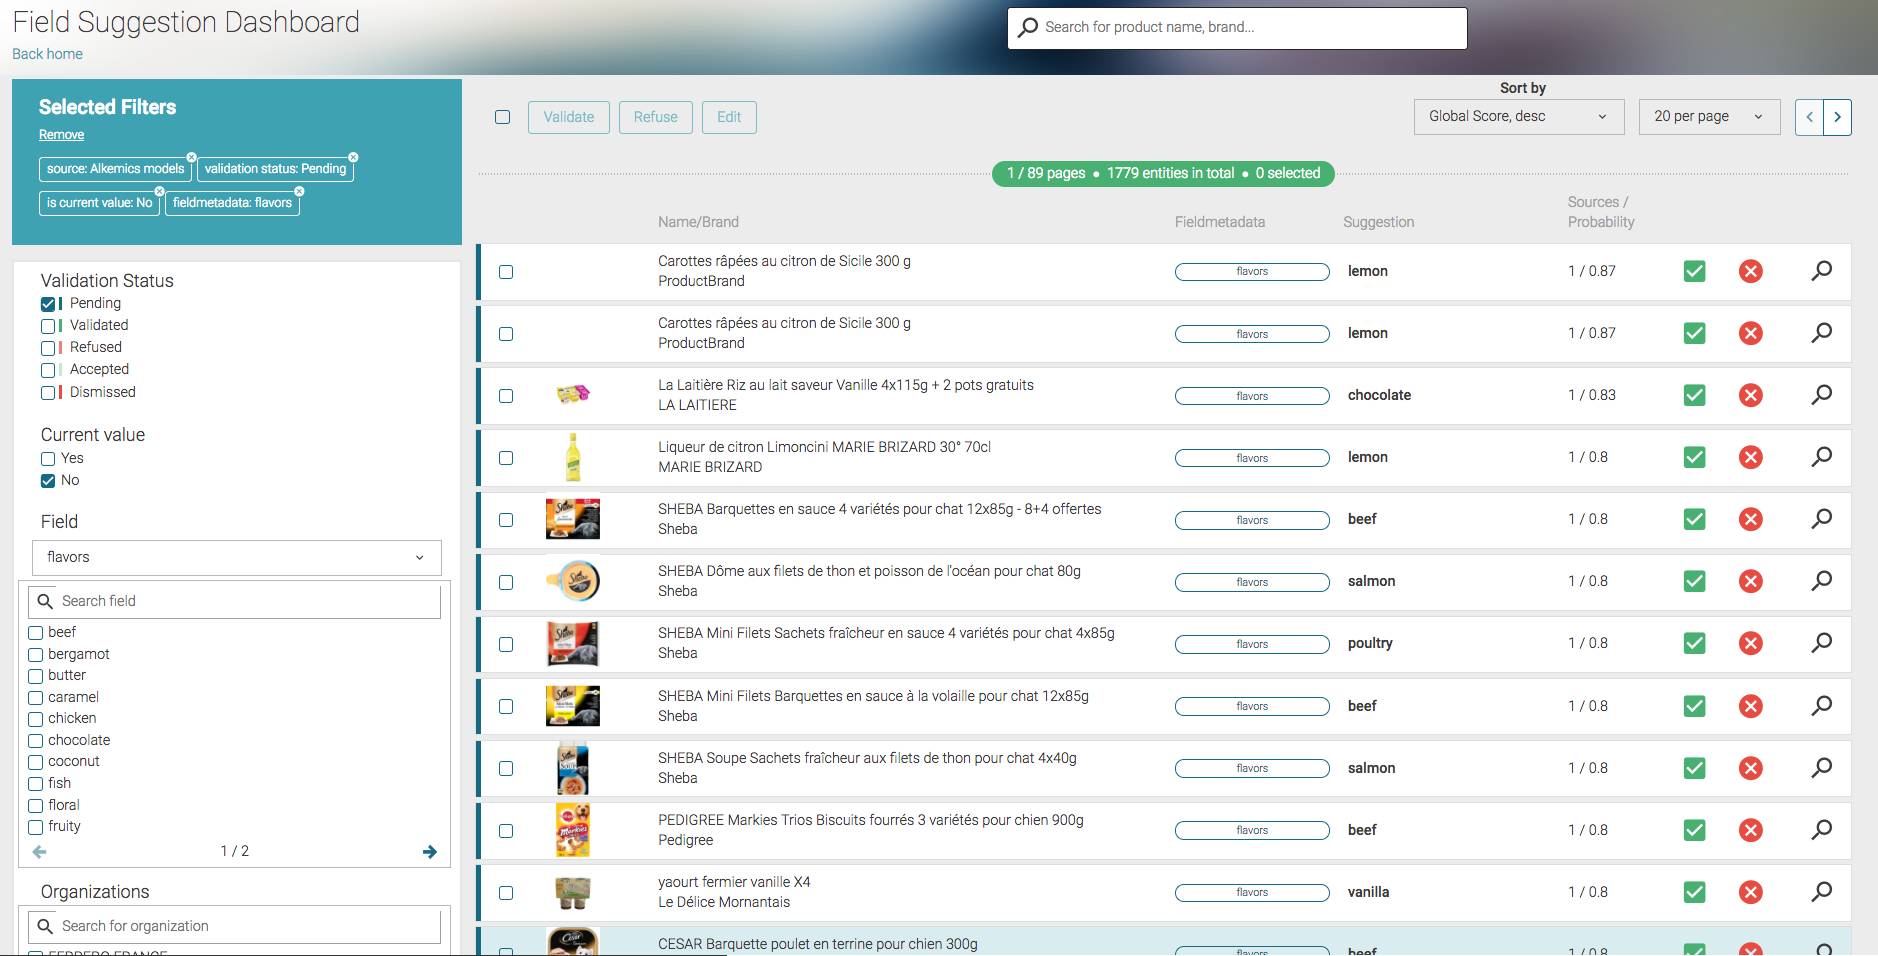
\includegraphics[scale=0.50]{./images/data-quality/validation-dashboard.png}
\caption{Validation dashboard.}
\end{figure}

This dashboard allows us to easily filter suggestions based on:
\begin{multicols}{2}
\begin{itemize} 
	\item validation/acceptation status
	\item is prediction a the current value
	\item field (flavors, kind...)
	\item classes (gluten, lactose...)
	\item organizations
	\item source 
	\item score 
\end{itemize}
\end{multicols}

For instance it is thus possible to easily select suggestions whose validation status is pending, and that do not match current values in database. We can then sort these suggestions by number of different sources and filter those with sufficient precision estimation, and validate suggestions in batches.


\subsection{Tune fasttext hyperparameters}

Each predicted field data-set has different charateristics:
\begin{itemize}
	\item number of different classes (5 to 175)
	\item classes disparity: some fields have very distinct classes, whereas some others have very related classes.
	\item label density (for multilabel): do your products have on average 1 label or 5 different labels
\end{itemize}

Then, each of these tasks might require different model hyper-parameters (those parameters will be detailed in the next chapter).
That's why we build a service on a dedicated machine whose goal is to find the best parameters.

\subsection{Bootstrap new classes/fields}

Everyday at Alkemics, clients use our plateform, and the data changes, lives. Thus, unlike in kaggle competition, our datasets evolves.
For instance, some new ingredients might appear, and at the beginning their low number of occurence might prevent the model to perform well.

\begin{figure}[H]
\centering
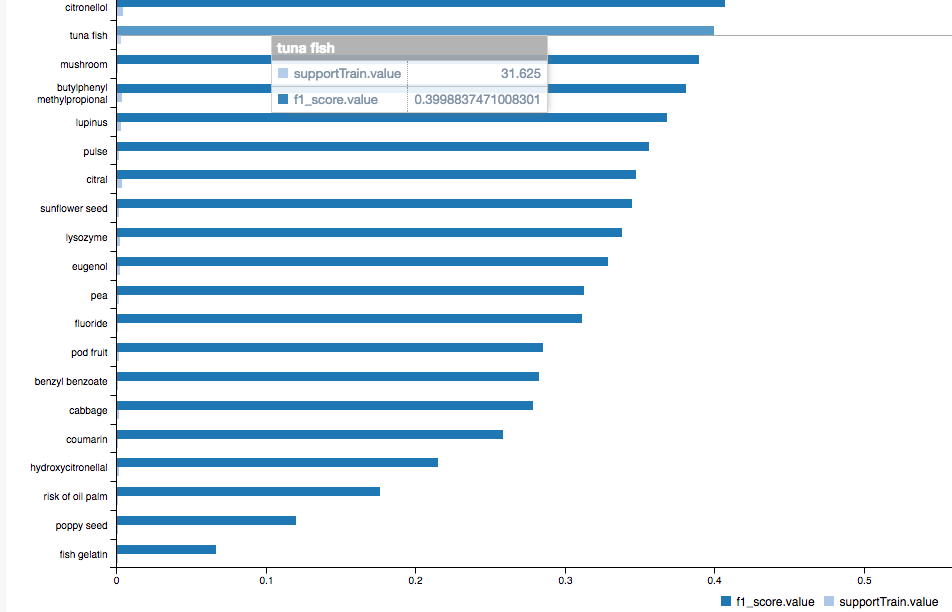
\includegraphics[scale=0.5]{./images/data-quality/islabeledby_support_score.png}
\caption{Selection of classes with lowest scores. Tuna fish performs badly, because of the low train support.}
\end{figure}

In that case we will use our validation dashboard. We would make a textual search to validate some related suggestions, or even create manually some suggestions. Sometimes, even some dozens of occurences will bootstrap a new class and launch a virtuous circle for the model.



\cleardoublepage
\chapter{Machine learning challenges}
\label{cha:results}


\section{Text categorization}

When dealing with natural language, one of the most important common denominator is how we represent words as input to any of our models. How do we transform sentences/words into numerical vectors.

In this section, we will quickly describe Mikolov's Word2Vec models (Continuous Bag of Word, and Skip-Gram), that proposed a new way to build word embeddings based on words coocurrence in a context window.

Then we will explain in more detail recent work from Facebook, that proposes new models based on Mikolov's work, allowing the use of sub-word information, and proposing a novel way to compute classification tasks while learning embeddings.

\subsection{Probability of sequence of tokens}

One solution to extract information from a corpus of text is to build a model that will assign a probability to a sequence of tokens. 

Let's consider the following sentence: \say{\textit{To classify you have to learn.}}

A good language model will give this sentence a high probability because this is a completely valid sentence, syntactically and semantically.

Similarly, the sentence \say{Before car bird eating sea.} should have a very low probability because it makes no sense. 

Mathematically, we can call this probability on any given sequence of n words:

\begin{align}
	P(\textit{'To'},\textit{'classify'}, ..., \textit{'learn'})
\end{align}

To make sense, we would like sentences of a given corpus to have a high probability.

Let's introduce the notations for this section:

{\ttfamily
\begin{table}[H]
    \centering
    \begin{tabular}{ll}
        \toprule
        $V$       	   	 &    the ordered vocabulary \\
        $T$    		   	 &    the size of corpus \\
        $w_i$          	 &    the i-th word in corpus \\
        $v_{i}$          	 &    the i-th word in vocabulary \\
        $V(w_i)$       &    the index of i-th word of corpus in vocabulary V, such as $ w_{i} = v_{V(w_i)}$\\
        $C_t^{(c)}$      &    the context of t-th word in corpus, for window of size $c$: $w_{t-c}, ..., w_{t-1}, w_{t+1}, ... ,w_{t+c}$\\
		$\mathbf{x}_i$ 				& one hot word vector corresponding i-th word in vocabulary $V$ \\
        $\mathbf{\bar x}$ 	& the average of all one hot vectors of words in context $C_t^{(c)}$ \\
        \bottomrule
    \end{tabular}
\end{table}
}

With:
\begin{align}
	\mathbf{x}_1 &= 
	\begin{bmatrix} 
		1 \\
		0 \\
		\vdots\\
		0
	\end{bmatrix} \\
	\mathbf{\bar x} &= \frac{\mathbf{x}_{V(t-c)} + \mathbf{x}_{V(t-c+1)} ... + \mathbf{x}_{V(t+c)}}{|C_t^{(c)}|}
\end{align}

Taking our corpus \say{\textit{To classify you have to learn.}}:

\begin{itemize}
	\item our corpus is of size: $T=6$
	\item our vocabulary is: $V =$ (to, classify, you, have, learn), an ordered list of size $|V| = 5$ (word \textbf{to} is present twice in corpus)
	\item $w_5$ is word \textbf{to}, indexed in vocabulary as $V(w_5) = 1$ (first word of vocabulary), ie $w_5 = v_1$
	\item $\mathbf{x}_{V(w_5)} = \mathbf{x}_{1} = \begin{bmatrix} 
		1 \\
		0 \\
		\vdots\\
		0
	\end{bmatrix}$
	\item $C_3^{(2)}$ is context of word \textbf{you} with window of size 2: \{to, classify, have, to\}
	\item 
		\begin{align}
		\mathbf{\bar x} &= (\mathbf{x}_{V(w_1)} +\mathbf{x}_{V(w_2)} + \mathbf{x}_{V(w_4)} + \mathbf{x}_{V(w_5)}) / 4 \\ 
		&= (\mathbf{x}_{1} +\mathbf{x}_{2} + \mathbf{x}_{4} + \mathbf{x}_{1}) / 4 
		=\begin{bmatrix} 
			1/2 \\
			1/4 \\
			0\\
			1/4\\
			0
		\end{bmatrix}
	\end{align}
\end{itemize}


\subsection{Word2Vec models}

Word2vec consists in either of two model architectures to produce a representation of words: \textbf{continuous bag-of-words} (CBOW) or \textbf{skip-gram}. 

In the continuous bag-of-words architecture, the model predicts the current word from a window of surrounding context words. The order of context words does not influence prediction (bag-of-words assumption). In the continuous skip-gram architecture, the model uses the current word to predict the surrounding window of context words. 
The skip-gram architecture weighs nearby context words more heavily than more distant context words.

Both models can be trained from an unlabeled large corpus of text and rely on the same trick: transform unlabeled data into a labeled dataset for supervised learning to unveil hidden dependencies between words.

Since these two models are quite similar, we will only describe in detail the CBOW in this section.

\subsubsection{CBOW}

In the CBOW model, we try to maximize the likelihood occurence of a word given its context, for a given window size.

Taking our previous corpus: \say{\textit{To classify you have to learn.}}


With a context window of size 2, we can extract many labeled samples:
\begin{itemize}
	\item \textbf{context}: \{classify, you\}, \textbf{target}: to
	\item \textbf{context}: \{to, you, have\}, \textbf{target}: classify
	\item \textbf{context}: \{to, classify, have, to\}, \textbf{target}: you
	\item ...
	\item \textbf{context}: \{have, to\}, \textbf{target}: learn
\end{itemize}


Mathematically, with $w_t$ our target word, $c$ the size of our context window, the probability of our target word given the context can be written as:

\begin{align}
	P(w_t | w_{t-c}, ..., w_{t-1}, w_{t+1}, ... ,w_{t+c}) = P(w_t | C_t^{(c)})
\end{align}

Given a word vocabulary of size $V$, the goal is to learn a vectorial representation for each word $w$. Word representations are trained to \emph{predict well} words that appear in its context.

So given a large training corpus represented as a sequence of words $w_1, ..., w_T$, the objective of the CBOW model is to maximize the following log-likelihood:
\begin{equation*}
  \sum_{t=1}^T \ \log P(w_t \ | \ \mathcal{C}_t^{(c)}),
\end{equation*}

\textbf{Parametrization and model}

The probability of observing a context word $w_t$ given $\mathcal{C}_t^{(c)}$ will be parameterized using the aforementioned word vectors.

We create two matrices $A \in \mathbb{R}^{dim \times |V|}$ and $B \in \mathbb{R}^{|V| \times dim}$, where $dim$ is an arbitrary size which defines the size of our embedding space.

$A$ is the input word matrix such that the i-th column of $A$ is the embedded vector of dimension \textit{dim} for word $v_{i}$ when it is an input to this model. 
Similarly, B is the output word matrix. The j-th row of B is an embedded vector of dimension \textit{dim} for word $v_j$ when it is an output of the model. 


Let's introduce some new notations:

{\ttfamily
\begin{table}[H]
    \centering
    \begin{tabular}{ll}
        \toprule
        $dim$ 				& chosen size for our embeddings \\
        $A$ 				& input word matrix $\in \mathbb{R}^{dim \times |V|}$ \\
        $B$ 				& output word matrix $\in \mathbb{R}^{|V| \times dim}$ \\
        \bottomrule
    \end{tabular}
\end{table}
}

The input matrix A converts our encoded input bag of words ($\mathbf{\bar x} $) into a representation in a lower dimensionality.

Let's denote our hidden representation:
\begin{align}
 \mathbf{h}_t = A.\mathbf{\bar x}
\end{align}

Finally, this hidden representation will be decoded with the output matrix B to be able to compare it with our target word. Since we are in a single labeled multiclass case, the use of softmax function is adapted to sum our probabilities to 1. In short, in CBOW we define the probability of occurence of each word of the vocabulary, given a context $\mathcal{C}_t^{(c)}$ (our model), as:

\begin{align}
 \mathbf{\hat y}_t = 
	\begin{bmatrix} 
		P(v_1 | \mathcal{C}_t^{(c)}) \\
		\vdots \\
		P(v_t | \mathcal{C}_t^{(c)})\\
		\vdots \\
		P(v_{|V|} | \mathcal{C}_t^{(c)})
	\end{bmatrix} = 
	softmax(B.A.\mathbf{\bar x} )
\end{align}

Ie $\forall i \in [1, |V|]$:
\begin{align}
 P(v_i | \mathcal{C}_t^{(c)})= 
 	&\frac{  [e^{B.A.\mathbf{\bar x}}]_i}
 	{\sum_{j=1}^{|V|} [e^{B.A.\mathbf{\bar x}} ]_j} \\
 	\text{      with}& []_i \text{ meaning the i-th element of a vector}
\end{align}


Whereas the true target is noted (target word in vocabulary):
\begin{align}
 \mathbf{y}_t = 
	\begin{bmatrix} 
		0 \\
		\vdots \\
		1 \\
		\vdots \\
		0
	\end{bmatrix} 
	= \mathbf{x}_{V(w_t)}
\end{align}


Since $\mathbf{y}_t$ is a one-hot vector (with 1 at location $V(w_t)$), maximizing log-likelihood of $P(w_t | \mathcal{C}_t^{(c)})$ is equivalent to minimizing the cross entropy of $(\mathbf{\hat y}_t, \mathbf{y}_t)$:
\begin{align}
E(\mathbf{\hat y}_t, \mathbf{y}_t) &= - \mathbf{y}_t^{\top} log(\mathbf{\hat y}_t) = - log(P(v_{V(w_t)} | \mathcal{C}_t^{(c)})) =- log(P(w_t | \mathcal{C}_t^{(c)}))
\end{align}

We can represent it as the following multilayer network:

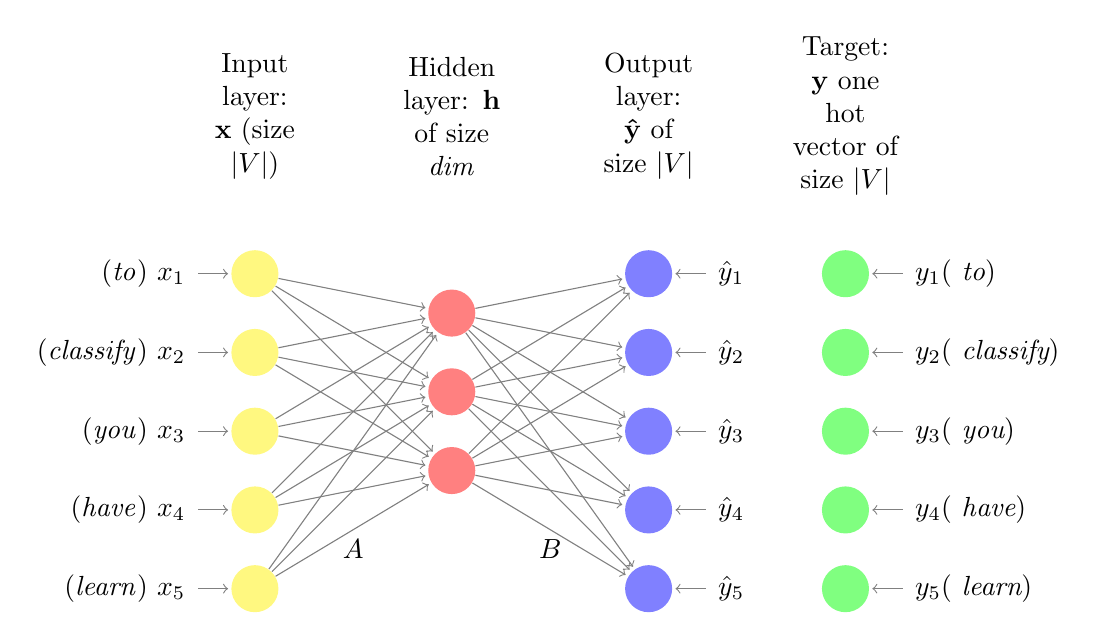
\begin{tikzpicture}[shorten >=1pt,->,draw=black!50, node distance=\layersep]
    \tikzstyle{every pin edge}=[<-,shorten <=1pt]
    \tikzstyle{neuron}=[circle,fill=black!25,minimum size=17pt,inner sep=0pt]
    \tikzstyle{input neuron}=[neuron, fill=yellow!50];
    \tikzstyle{output neuron}=[neuron, fill=blue!50];
    \tikzstyle{hidden neuron}=[neuron, fill=red!50];
    \tikzstyle{true neuron}=[neuron, fill=green!50];
    \tikzstyle{annot} = [text width=4em, text centered]

    % Draw the input layer nodes
    \foreach \name / \y / \word in {1/1/to,2/2/classify,3/3/you,4/4/have,5/5/learn}
        \node[input neuron, pin=left: (\textit{\word}) $x_{\y}$ ] (I-\name) at (0,-0.5 -\y) {};

    % Draw the hidden layer nodes
    \foreach \name / \y in {1,...,3}
        \node[hidden neuron] (H-\name) at (\layersep,-1 -\y) {};
    
    % Draw the output layer node

	\foreach \name / \y in {1,...,5}
        \node[output neuron, pin=right:$\hat y_{\y}$ ] (O-\name) at (\layersep*2,-0.5 -\y) {};

    % Draw the true layer node
	\foreach \name / \y / \word in {1/1/to,2/2/classify,3/3/you,4/4/have,5/5/learn}
        \node[true neuron, pin=right:$y_{\y} (\textit{  \word})$ ] (T-\name) at (\layersep*3,-0.5 -\y) {};


    % Connect every node in the input layer with every node in the
    % hidden layer.
    \foreach \source in {1,...,5}
        \foreach \dest in {1,...,3}
            \path (I-\source) edge (H-\dest);

    % Connect every node in the hidden layer with the output layer
    \foreach \source in {1,...,3}
        \foreach \dest in {1,...,5}
	        \path (H-\source) edge (O-\dest);

    % Annotate the layers
    \node[annot,above of=H-1, node distance=2.5cm] (hl) {Hidden layer: $\mathbf{h}$ of size \textit{dim}};
    \node[annot,left of=hl] {Input layer: $\mathbf{x}$ (size $|V|$)};
    \node[annot,right of=hl] (ol) {Output layer: $\mathbf{\hat y}$ of size $|V|$};
    \node[annot,right of=ol] {Target: $\mathbf{y}$ one hot vector of size $|V|$};

    \node[annot] (A) at (\layersep/2,-5) {$A$};
    \node[annot] (B) at (\layersep*3/2,-5) {$B$};

\end{tikzpicture}

Matrices A and B are updated using gradient descent and gradient retro-propagation.

\subsubsection{Using CBOW embeddings for classification}

Using CBOW algorithm would provide you this A matrix, which is basically a lookup table in which you can extract the representation of any word of your vocabulary in your embedding space (of size $dim <<< |V|$).

Word2Vec treats each word in corpus like an atomic entity and generates a vector for each word.

Transforming a text input in a numerical vector is then possible, and your numerical vector could then be used as input for any classification algorigthm to perform classification tasks.

\subsection{Fasttext}

Fasttext, which is essentially an extension of word2vec model, brings two major conceptual changes (in addition to a very efficient C++ implementation):
\begin{itemize}
	\item simulatenous embedding and classification learning: in Word2Vec, we first build our embeddings, and then use it to translate words in features of low dimensionality for further classification. In fasttext, embedding and classification are different layers of a neural network that are trained simultaneously.
	\item use of subword word information, instead of treating only word entities
\end{itemize}

Details can be found in two papers published by Fasttext team: \cite[Enriching Word Vectors with Subword Information]{fasttextEnriching} and \cite[Bag of Tricks for Efficient Text Classification]{fasttextTricks}

\subsubsection{Multiclass classification model}

Let's consider the case where we have a training set of multiclass single-labeled sentences, for instance:
\begin{itemize}
	\item \textbf{feature}: \{I'm hungry\}, \textbf{target}: neutral 
	\item \textbf{feature}: \{Get out\}, \textbf{target}: angry
	\item \textbf{feature}: \{Nice to be there\}, \textbf{target}: happy
	\item ...
	\item \textbf{feature}: \{Do you want this apple\}, \textbf{target}: curious
\end{itemize}
With our target space being: \{happy, angry, neutral, curious\}, of size $K=4$

What fasttext does, is that instead of first learning word embeddings on a corpus of text, it directly uses features to build specialized embeddings for this classification task.

Denoting $\mathcal{Y} = \{y_i\}_{i \in [1, K]}$, and $\mathbf{x}$ the average of one hot-encoded vector of tokens of a feature in vocabulary $V$:
\begin{align}
 \mathbf{\hat y} 
 = 
	\begin{bmatrix} 
		\hat y_1 \\
		\vdots \\
		\hat y_i\\
		\vdots \\
		\hat y_K
	\end{bmatrix} 
 =	\begin{bmatrix} 
		P(y_1 | \mathbf{x}) \\
		\vdots \\
		P(y_i | \mathbf{x})\\
		\vdots \\
		P(y_K | \mathbf{x})
	\end{bmatrix} = 
	softmax(B.A.\mathbf{x})
\end{align}

Ie $\forall i \in [1, K]$:
\begin{align}
 P(y_i | \mathbf{x})= 
 	&\frac{  [e^{B.A.\mathbf{x}}]_i}
 	{\sum_{j=1}^{K} [e^{B.A.\mathbf{x}}]_j} \\
 	\text{      with}& []_i \text{ meaning the i-th element of a vector}
\end{align}


Whereas the true target is noted:
\begin{align}
 \mathbf{y} = 
	\begin{bmatrix} 
		y_1 \\
		\vdots \\
		y_i \\
		\vdots \\
		y_K
	\end{bmatrix} 
\end{align}
wich is a one hot encoded vector corresponding to which is this sample label.


The model is very similar to continuous bag of words model, except that instead of using the middle word of CBOW, we directly use a label. The architecture is then:
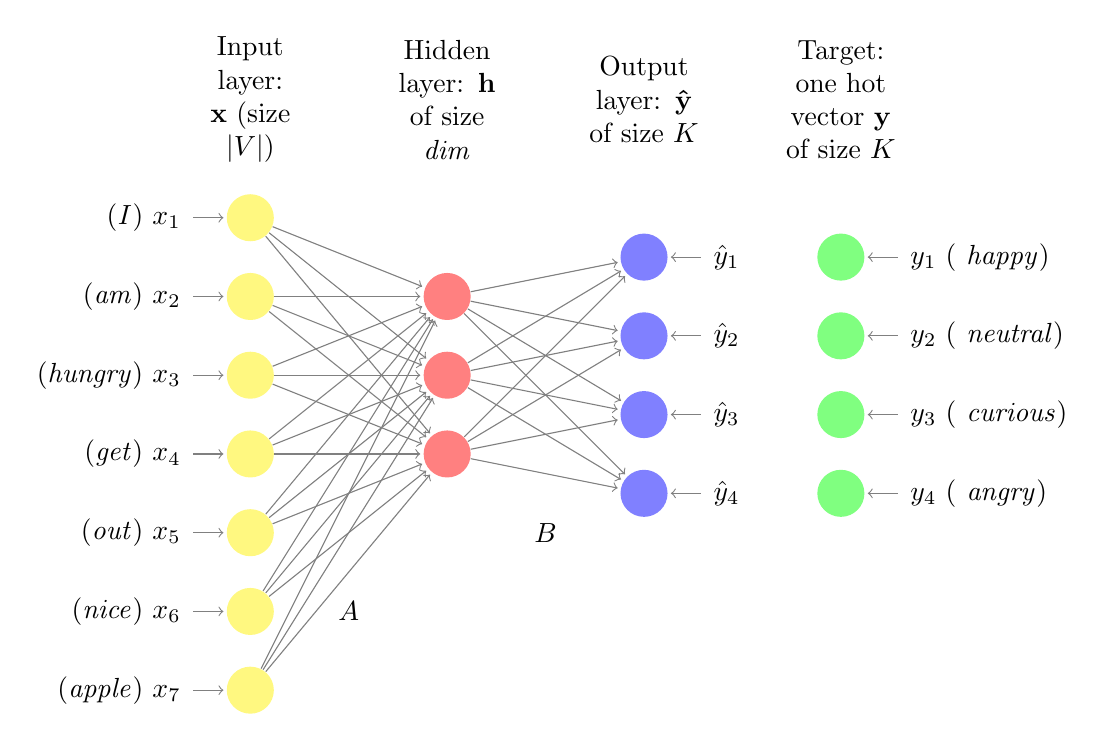
\begin{tikzpicture}[shorten >=1pt,->,draw=black!50, node distance=\layersep]
    \tikzstyle{every pin edge}=[<-,shorten <=1pt]
    \tikzstyle{neuron}=[circle,fill=black!25,minimum size=17pt,inner sep=0pt]
    \tikzstyle{input neuron}=[neuron, fill=yellow!50];
    \tikzstyle{output neuron}=[neuron, fill=blue!50];
    \tikzstyle{hidden neuron}=[neuron, fill=red!50];
    \tikzstyle{true neuron}=[neuron, fill=green!50];
    \tikzstyle{annot} = [text width=4em, text centered]

    % Draw the input layer nodes
    \foreach \name / \y / \word in {1/1/I,2/2/am,3/3/hungry,4/4/get,5/5/out, 6/6/nice, 7/7/apple}
        \node[input neuron, pin=left:(\textit{\word  }) $x_{\y}$ ] (I-\name) at (0,-\y) {};

    % Draw the hidden layer nodes
    \foreach \name / \y in {1,...,3}
        \node[hidden neuron] (H-\name) at (\layersep,-1 -\y) {};

    % Draw the output layer node
	\foreach \name / \y in {1,...,4}
        \node[output neuron, pin=right:$\hat y_{\y}$ ] (O-\name) at (\layersep*2,-0.5 -\y) {};

    % Draw the true layer node
	\foreach \name / \y / \label in {1/1/happy,2/2/neutral, 3/3/curious,4/4/angry}
        \node[true neuron, pin=right:$y_{\y}$ (\textit{  \label})] (T-\name) at (\layersep*3,-0.5 -\y) {};

    % Connect every node in the input layer with every node in the hidden layer.
    \foreach \source in {1,...,7}
        \foreach \dest in {1,...,3}
            \path (I-\source) edge (H-\dest);

    % Connect every node in the hidden layer with the output layer
    \foreach \source in {1,...,3}
        \foreach \dest in {1,...,4}
	        \path (H-\source) edge (O-\dest);

    % Annotate the layers
    \node[annot,above of=H-1, node distance=2.5cm] (hl) {Hidden layer: $\mathbf{h}$ of size \textit{dim}};
    \node[annot,left of=hl] {Input layer: $\mathbf{x}$ (size $|V|$)};
    \node[annot,right of=hl] (ol) {Output layer: $\mathbf{\hat y}$ of size $K$};
    \node[annot,right of=ol] {Target: one hot vector $\mathbf{y}$ of size $K$};

    \node[annot] (A) at (\layersep/2,-6) {$A$};
    \node[annot] (B) at (\layersep*3/2,-5) {$B$};

\end{tikzpicture}
Note: 
\begin{itemize}
	\item for readibility just 7 words of the input features are considered.
	\item fasttext first merge all features as one corpus to build vocabulary ($\rightarrow$ size of matrix A)
	\item in practice, dimension of the hidden layer is between 50 and 300
	\item input matrix A embeddings are specialized for this classification task and may not behave well for another classification task
	\item the target vector is exactly composed of one 1, and the rest of 0s (multi-class).
\end{itemize}

\textbf{Subword information}

Each word can be considered as a set of character ngrams. In Fasttext, a word vector is made of the sum of this character n grams. For example the word vector “apple” is a sum of the vectors of the n-grams:
\begin{multicols}{4}
\begin{itemize}
	\item “<ap”, 
	\item “app”, 
	\item ”appl”, 
	\item ”apple”, 
	\item ”apple>”, 
	\item “ppl”, 
	\item “pple”, 
	\item ”pple>”, 
	\item “ple”, 
	\item ”ple>”, 
	\item ”le>”
\end{itemize}
\end{multicols}
Note: this behavious is controlled through hyperparameters controlling smallest ngram size ([minn]) and largest ngram size ([maxn]). For performance and memory size reasons, another hyperparameter ([bucket]) controls the maximum total number of tokens (word tokens + subword tokens).

This provide the following advantages:
\begin{itemize}
	\item Generate better word embeddings for rare words (even if words are rare their character n grams are still shared with other words - hence the embeddings can still be good). In word2vec a rare word (e.g. 10 occurrences) has fewer neighbors to be tugged by, in comparison to a word that occurs 100 times - the latter has more neighbor context words and hence is tugged more often resulting in better word vectors.
	\item Out of vocabulary words - they can construct the vector for a word from its character n grams even if word doesn't appear in training corpus. The choice of hyper parameters controlling the minimum and maximum n-gram sizes has to be chosen.
\end{itemize}

Concretely, the use of subword information will only impact:
\begin{itemize}
	\item how is built the vocabulary. It will not only contain words of the training corpus, but also all ngrams of these words. The vocabulary will thus be much bigger, but with shared properties between different words.
	\item how features are encoded in this vocabulary: 'Do you want this apple' will not be encoded as the average of 5 one hot vectors \{do, you, want, this, apple\}, but as the average of one hot vectors of all tokens contained in the sentence \{<do>, <you, you>, <wa, wan, ant, nt> ...\}.
\end{itemize}

\subsubsection{Miscellanous}

Optimization, hierarchical softmax, negative sampling, word-n-grams, text preprocessing etc..


\pagebreak
\section{Multilabel classification}

We already studied in previous section how we could compute efficient multi-class classification from natural language input. Yet in our project, most of the product attributes that we wanted to predict were multi-labeled.

In this section, we will first make a quick review of the major algorithms and scoring metrics for multi-label classification, mainly based on the ~\cite[following paper]{MultilabelReview}. Then we will focus on another common approach in neural networks not detailed in the previous paper, that inspired us to modify fasttext algorithm to make it natively support multilabel classification.


\subsection{Multilabel metrics}

Suppose $\mathcal{X} = \mathbb{R}^d$ denotes the \textit{d}-dimensional instance space, and  $\mathcal{Y} = \{y_1, y_2, \dots, y_K \}$ the label space with $K$ possible class labels.

Let's denote $\mathcal{D} = \{(\mathbf{x}_i, Y_i) | 1 \leq i \leq n\}$ our learning dataset. For each multi-label example $(\mathbf{x}_i, Y_i)$, $Y_i \subseteq \mathcal{Y}$ is the set of labels for $\mathbf{x}_i$.

\subsubsection{Common dataset description metrics}

\begin{itemize}
	\item \textbf{Number of classes}: $|\mathcal{Y}| = K$.
	\item \textbf{Label cardinality}: $\frac{1}{n}\sum_{i=1}^n |Y_i|$ (average number of labels per sample).
	\item \textbf{Label density}: $\frac{1}{n \times |\mathcal{Y}|}\sum_{i=1}^n |Y_i|$ (average number of labels per example normalized by number of classes).
	\item \textbf{Label diversity}: $|\{Y | \exists \mathbf{x}:(\mathbf{x}, Y) \in \mathcal{D}\}|$ (the number of distinct label sets in learning set).
\end{itemize}


\subsubsection{Scoring metrics}

In multi-label context, scoring metrics can be divided in two groups \cite{MultilabelReview}: 
\begin{itemize}
	\item sample-wise metrics: how well we performed on a sample
	\item label-wise metrics: how well we performed on a given class
\end{itemize}

In our case, the metrics of most interest are label-wise metrics, we will detail those we consider, which are derived from binary classification scoring metrics.  

Denoting $f$ our classifier, let's define the following metrics, for each class independently:
$\forall j \in [1, K]$:
{\ttfamily
\begin{table}[H]
    \centering
    \begin{tabular}{ll}
        \toprule
        $TP_j = |\{ \mathbf{x}_i | y_j \in Y_i \wedge y_j \in f(\mathbf{x}_i), 1 \leq i \leq n \}|$          &    $true\ positives\ for\ class\ j$ \\
        $FP_j = |\{ \mathbf{x}_i | y_j \notin Y_i \wedge y_j \in f(\mathbf{x}_i), 1 \leq i \leq n \}|$          &    $false\ positives\ for\ class\ j$ \\
        $TN_j = |\{ \mathbf{x}_i | y_j \notin Y_i \wedge y_j \notin f(\mathbf{x}_i), 1 \leq i \leq n \}|$       &    $true\ negatives\ for\ class\ j$  \\
        $FN_j = |\{ \mathbf{x}_i | y_j \in Y_i \wedge y_j \notin f(\mathbf{x}_i), 1 \leq i \leq n \}|$       &    $false\ negatives\ for\ class\ j$  \\
        \bottomrule
    \end{tabular}
\end{table}
}

Let $B(TP_j, FP_j, TN_j, FN_j)$ represent some binary classification metric among those of most interest for us: Precision, Recall, $F_{\beta}$ score (detailed in appendix). 

These metrics can be considered as \textit{local} metrics: each is specific to a given class. To obtain what we can could call \textit{global} metrics, that represent performance on all classes, two kinds of averaging can be considered:

\begin{itemize}
	\item Macro-averaging: equal weights for labels.
	\begin{align}
		B_{macro}(h) = \frac{1}{K}\sum_{j=1}^K B(TP_j, FP_j, TN_j, FN_j)
	\end{align}
	\item Micro-averaging: equal weights for samples.
	\begin{align}
		B_{micro}(h) = B(\sum_{j=1}^K TP_j, \sum_{j=1}^K FP_j,\sum_{j=1}^K  TN_j,\sum_{j=1}^K  FN_j)
	\end{align}
\end{itemize}


Those two averaging answer to different challenges. A high micro-averaged score can hide very poor results on classes with few occurences. A high macro-averaged score will give the same impact for a class with 1000 samples and another class of 2 samples. Both have their benefits and weaknesses depending on your goal.

In our case, our interest was more focused on micro-averaging, and classes with too poor local metrics are filtered after prediction.

\subsection{Output size challenge}

The key challenge of learning from multi-label data lies in the overwhelming size of output space, i.e. the number of label sets grows exponentially as the number of class labels increases. For example, for a label space with 20 class labels, the number of possible label sets would exceed one million ($2^{20}$).

Existing strategies to label correlations exploitation can be categorized based on the order of correlations that the learning techniques have considered:
\begin{itemize}
	\item First-order strategy: The task of multi-label learning is tackled in a label-by-label style and thus ignoring co-existence of the other labels, such as decomposing the multi-label learning problem into a number of independent binary classification problems (one per label). 
	\item Second-order strategy: The task of multi-label learning is tackled by considering pairwise relations between labels, such as the ranking between relevant label and irrelevant label , or interaction between any pair of labels, etc.
	\item High-order strategy: The task of multi-label learning is tackled by considering high-order relations among labels such as imposing all other labels’ influences on each label, or addressing connections among random subsets of labels, etc.
\end{itemize}

There is a compromise to find between taking into account correlations between labels, or choosing computational efficiency: the computational complexity quickly increase.

\subsection{Multi-label learning algorithms}

Multilabel strategies can be grouped in two main approaches: problem transformation methods or algorithm adaptation methods.

Briefly, the key philosophy of problem transformation methods is to fit data to algorithm,
while the key philosophy of algorithm adaptation methods is to fit algorithm to data. Figure ~\ref{fig:multilabelOverview}
summarizes the algorithms detailed in \cite[Zhang and Zhou paper]{MultilabelReview}.

\textbf{Algorithm adaptation methods}

This category of algorithms tackle multi-label learning problem by adapting popular learning techniques to deal with multi-label data directly. Each technique is thus specific to one algorighm.
Some adaptative algorithm exist for lazy learning techniques (kNN), decision tree techniques, kernel techniques (SVM), information-theoretic techniques (CRF).

\textbf{Problem transformation methods}

This category of algorithms tackle multi-label learning problem by transforming it into other well-established learning scenarios (binary or multiclass classification scenarios). 
Representative algorithms include:
\begin{itemize}
 \item first-order approaches Binary Relevance which transform the task of multi-label learning into the task of binary classification 
 \item high-order approach Classifier Chains which transform the task of multi-label learning into the task of binary classification 
 \item secondorder approach Calibrated Label Ranking which transforms the task of multi-label learning into the task of label ranking
 \item high-order approach Random k-labelsets which transforms the task of multi-label learning into the task of multi-class classification
\end{itemize}

\begin{figure}[H]
\centering
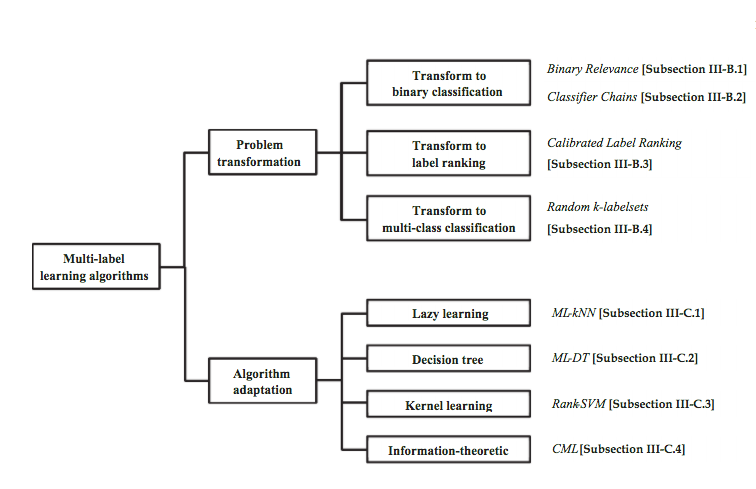
\includegraphics[scale=0.6]{./images/machine-learning/multi-label-approaches.png}
\caption{Categorization of representative multi-label learning algorithms reviewed in \cite[this paper]{MultilabelReview}.}
\label{fig:multilabelOverview}
\end{figure}


\subsection{Considered approaches}

In our case, the possible approaches were:
\begin{itemize}
	\item 'Word Embedding / Multi-label Classification':
	\begin{itemize}
		\item first learn general purpose word embeddings
		\item and then apply any multi-label classifier strategy
	\end{itemize}
	\item 'Fasttext / Problem Transform approach'
	\begin{itemize}
		\item use fasttext as binary/multiclass classifier
		\item as input for a problem transform approach: binary relevance, random-k-labelsets (classifier chains was not adaptable to fasttext)
	\end{itemize}
	\item adapt fasttext to support multi-label: learn simultanously embeddings and classifier parameters in multilabel context
\end{itemize}

\subsubsection{Project constraints}


Our first experiments with Fasttext encouraged us to try to use it. Reasons for that choice were:
\begin{itemize}
	\item subword ability
	\item encouraging scores
	\item training speed
	\item small RAM consumption
	\item quality of implementation
	\item well maintained code
\end{itemize}

TODO: from Spark to python

Since we knew that the multi-labeled attributes we wanted to predict are insufficiently labeled, we wanted a fast to train model that could be computed regularly (daily). Because of the iterative improvement and daily evolution of our products data. 

\begin{itemize}
	\item wanted to have same language in the whole pipeline (previously spark)
	\item run fitting on single machine
	\item prepare real-time prediction

\end{itemize}

\subsection{How we adapted Fasttext to multilabel}

Basically, the idea is to replace the last layer, from multiclass logistic regression to multi-binary logistic regression. Changes include:

\begin{itemize}
	\item the target vector is no longer one-hot encoded but can be any vector made of 0s and 1s.
	\item instead of applying a softmax function to output scores, we apply the logistic/sigmoïd function
	\item we use the logistic loss to update gradients
\end{itemize}


Denoting $\sigma$ the sigmoïd function:

\begin{align}
	\sigma(z) = \frac{1}{1 + \exp(-z)}
\end{align}

\begin{align}
 \mathbf{\hat y}
 	= \begin{bmatrix} 
		\hat y_1 \\
		\vdots \\
		\hat y_i\\
		\vdots \\
		\hat y_K
	\end{bmatrix}
	 = \begin{bmatrix} 
		P(y_1 | \mathbf{x}) \\
		\vdots \\
		P(y_i | \mathbf{x})\\
		\vdots \\
		P(y_K | \mathbf{x})
	\end{bmatrix} = 
	\sigma(B.A.\mathbf{x})
\end{align}

For all $i \in [1, K]$: 
\begin{align}
	P(y_i | \mathbf{x}) &= \frac{1}{1 + e^{[B.A.\mathbf{x}]_i}}\\
		\text{      with } &[z]_i \text{ meaning the i-th element of a vector}
\end{align}

Whereas the true target is noted (binary vector):
\begin{align}
 \mathbf{y} = 
	\begin{bmatrix} 
		y_1 \\
		\vdots \\
		y_i \\
		\vdots \\
		y_K
	\end{bmatrix}
	= 
	\begin{bmatrix} 
		0 \\
		1 \\
		1 \\
		\vdots \\
		0
	\end{bmatrix}  
\end{align}

Based on the assumption that $\mathbf{y}$ components are independent, (which is unfortunatly usually false but lets us treat each class independently as a binary problem), minimizing the following loss on one sample $(\mathbf{x}, \mathbf{y})$ is equivalent to maximizing log-likelihood:

\begin{align}
	E = - \sum_{k=1}^K
  			  	\left\{
				    \begin{array}{ll}
				        \log (\hat y_k) & \mbox{if } y_k =1 \\
				        \log (1 - \hat y_k) & \mbox{if } y_k =0
				    \end{array}
				\right.
\end{align}

Demonstration is present in appendix A.


\subsubsection{Gradient retropropagation}

Let's introduce some more notations that will help to compute gradients.

\begin{align}
	\mathbf{h}
	= \begin{bmatrix} 
		h_1 \\
		h_2 \\
		\vdots \\
		h_{\textit{dim}}
	\end{bmatrix}
	= A\mathbf{x}
\end{align}

With:
\begin{align}
	h_j = A^{(j)}\mathbf{x}
\end{align}


Let's denote:

\begin{align}
	s_k  = B^{(k)} \mathbf{h} = \sum_{j=1}^{\textit{dim}} B^{(k)}_j h_j 
\end{align}

we can then express $\hat y$ as, $\forall k \in [1, K]$:

\begin{align}
	\hat y_k  = \sigma(s_k) = \sigma( \sum_{j=1}^{d} B^{(k)}_j h_j) 
\end{align}


The gradient are:

\begin{align}
	\frac{ \partial E } { \partial \hat y_k } = 
		\left\{
		    \begin{array}{ll}
		        - \frac{1}{\hat y_k} & \mbox{if } y_k =1 \\
		        \frac{1}{1 - \hat y_k} & \mbox{if } y_k =0
		    \end{array}
		\right.
\end{align}


\begin{align}
	\frac{ \partial E } { \partial s_k } 
		=  
		\frac{ \partial E } { \partial \hat y_k } \cdot \frac{ \partial \hat y_k } { \partial s_k } 
		&=
		\left\{
		    \begin{array}{ll}
		        - \frac{1}{\hat y_k} \cdot \hat y_k (1 - \hat y_k)& \mbox{if } y_k =1 \\
		        \frac{1}{1 - \hat y_k} \cdot \hat y_k (1 - \hat y_k)& \mbox{if } y_k =0
		    \end{array}
		\right. \\
		&=
		\left\{
		    \begin{array}{ll}
		       \hat y_k - 1 & \mbox{if } y_k =1 \\
		       \hat y_k & \mbox{if } y_k =0
		    \end{array}
		\right. \\
		&= \hat y_k - y_k
\end{align}



\begin{align}
	\frac{\partial E}{\partial B_i^{(k)}} 
	= 
	\frac{\partial E}{\partial s_k} \cdot \frac{\partial s_k}{\partial B_i^{(k)}} 
	= 
	h_i (\hat y_k - y_k)
\end{align}


Trick: derivate $E$ in regard to $s_k$:
\begin{align}
	\frac{\partial E}{\partial h_j} 
	&= 
	\sum_{k=1}^K \frac{\partial E}{\partial s_k} \cdot \frac{\partial s_k}{\partial h_j} \\
	&= 
	\sum_{k=1}^K B_j^{(k)} (\hat y_k - y_k)
\end{align}


\begin{align}
	\frac{\partial E}{\partial A_i^{(j)}} 
	&= 
	\frac{\partial E}{\partial h_j} \cdot \frac{\partial h_j}{\partial A_i^{(j)}} \\
	&= 
	x_i \sum_{k=1}^K B_j^{(k)} (\hat y_k - y_k)
\end{align}


\subsubsection*{Gradient descent}

At each sample $(\mathbf{x}, \mathbf{y})$, given a learning rate $\mu$, we update weights as follow:

\begin{align}
	B_i^{(k)\mbox{new}} \leftarrow B_i^{(k)\mbox{old}} - \mu (h_i (\hat y_k - y_k))
\end{align}

\begin{align}
	A_i^{(j)\mbox{new}} \leftarrow A_i^{(j)\mbox{old}} - 
	\mu 
	\left(
		x_i \sum_{k=1}^K B_j^{(k)\mbox{new}} (\hat y_k - y_k) 
	\right)
\end{align}

\subsection{Results}

Considering how simple is Fasttext linear classifier, results can be considered as good:
\begin{itemize}
	\item detail about achievements
\end{itemize}





\pagebreak
\section{Calibration}

When performing classification one often wants not only to predict the class label, but also to obtain a probability of the respective label. This probability gives some kind of confidence on the prediction.
Well calibrated classifiers are probabilistic classifiers for which the score output can be directly interpreted as a confidence level. For instance, a well calibrated (binary) classifier should classify the samples such that among the samples to which it gave a score close to 0.8, approximately 80\% actually belong to the positive class.

In our prediction process, having high training scores is important. But since we want to validate predictions before sending suggestions to our customers, it is even more important to have calibrated probabilities in order to estimate a prediction likelihood to be valid and easily and quickly validate of refuse it.

After producing our first predictions, we soon realized that we needed more control on scores computed by our models, even though the logistic regression naturally provides quite well calibrated scores:
\begin{itemize}
	\item for some classes, a 0.8 score would on average be right 0.5 of the time
	\item on other classes it could be the opposite, a 0.5 score could be right 0.8 of the time on average
\end{itemize}

\textbf{Calibration plot}

Calibration plot is a method that shows us how well the classifier is calibrated \cite{Calibration}: $$x\ axis = true\ probability,\ y\ axis=predicted\ probability$$

True probabilities are calculated for (sub)sets of examples with the same predicted score $P(y=1|X) \in [c-\delta, c+\delta]$: $$ p_{true}^c = \frac{P_{sub}^c}{P_{sub}^c + N_{sub}^c}$$ with $P_{sub}^c, N_{sub}^c$ being the proportion on positives and negative examples in a given subset with predicted probabilities $[c-\delta, c+\delta]$. The calibration plot of a perfectly calibrated classifier will be a diagonal.



In this section we will first present a naïve calibration we implemented, and then introduce more commonly adopted strategies.

\subsection{Naïve calibration}

\begin{figure}[H]
\centering
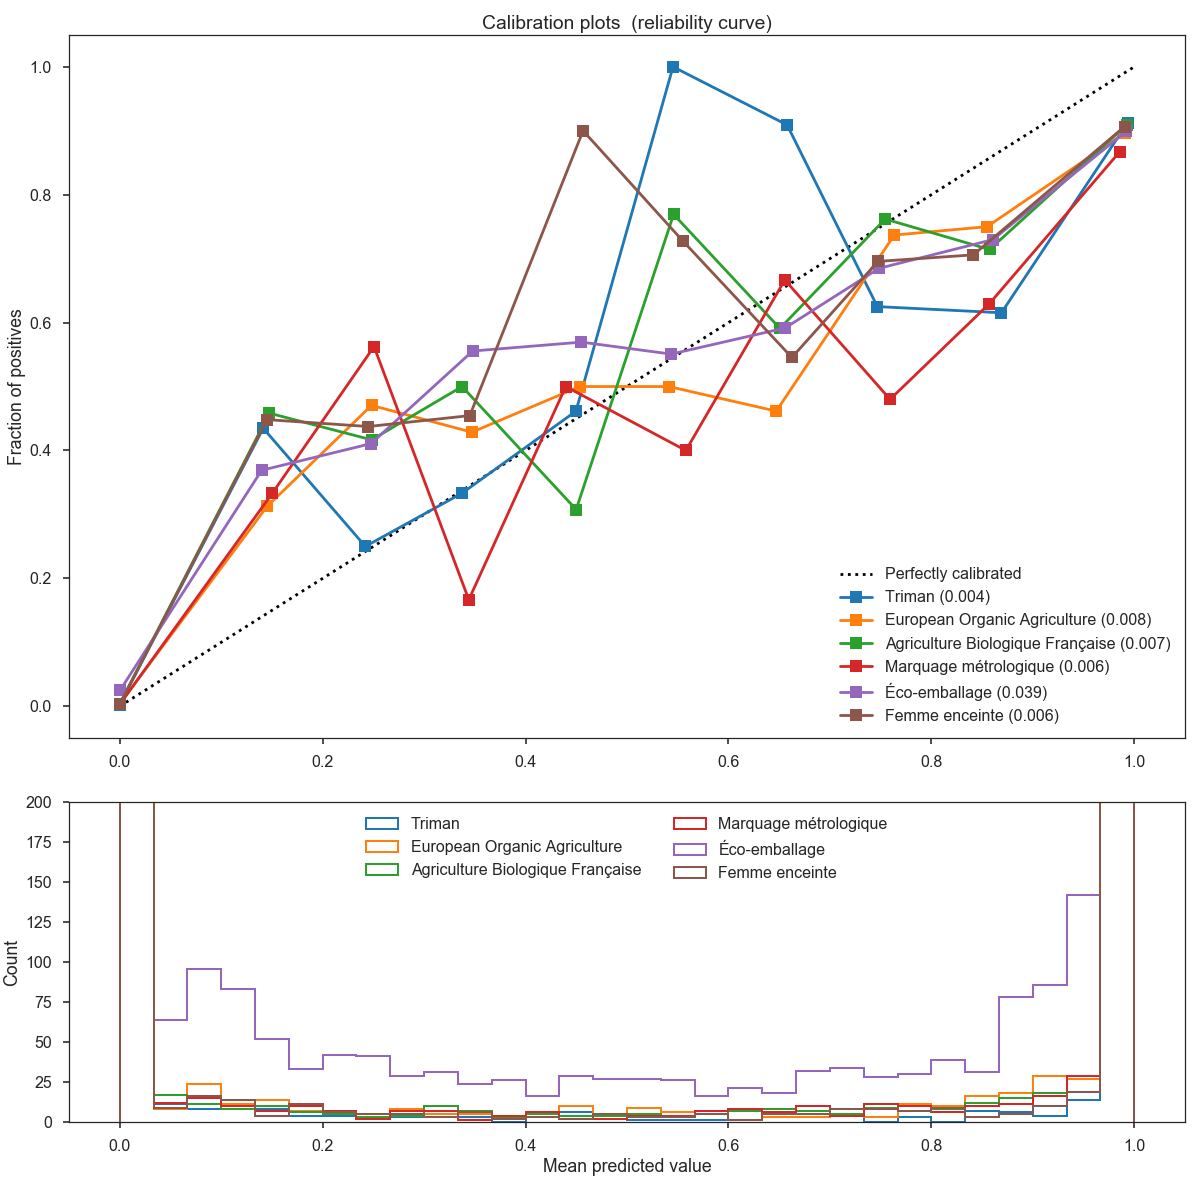
\includegraphics[scale=0.40]{./images/calibration/islabeledby_calibration_curve.png}
\caption{Calibration curve: true precision compared to predicted probabilities/scores.}
\end{figure}

One possible naïve solution would be to build bins of samples around a given score, for instance all scores between 0.40 and 0.50, and estimate the precision of samples in this bin (all prediction whose scores is between 0.4 and 0.5), as the mean precision of that bin on a validation data-set.

\subsection{More advanced calibration techniques}

Major approaches for performing calibration of probabilistic predictions share the same idea: use obtained classification scores as features in an additional classifier (classifier providing scores). We could cite: 
\begin{itemize}
	\item a parametric approach based on Platt’s sigmoid model: basically applying a logistic regression using classification scores as features, and original labels of a validation set as target \cite{Calibration}.
	\item a non-parametric approach based on isotonic regression: the idea is to fit a piecewise-constant non-decreasing function (stair-step shaped) instead of logistic regression (but the idea is similar to Platt's approach).
	\item a 'stacking-style' approach using classification scores as feature, but target are no longer original labels, but the thresholds bipartitioning labels with minimum misclassifications \cite{MultilabelReview}.
\end{itemize}

In our case, we tryed some Platt's and stacking-style calibration techniques, yet given the low label density of our training set, we overfit.

\subsection{Decision: precision versus recall}

\begin{figure}[H]
\centering
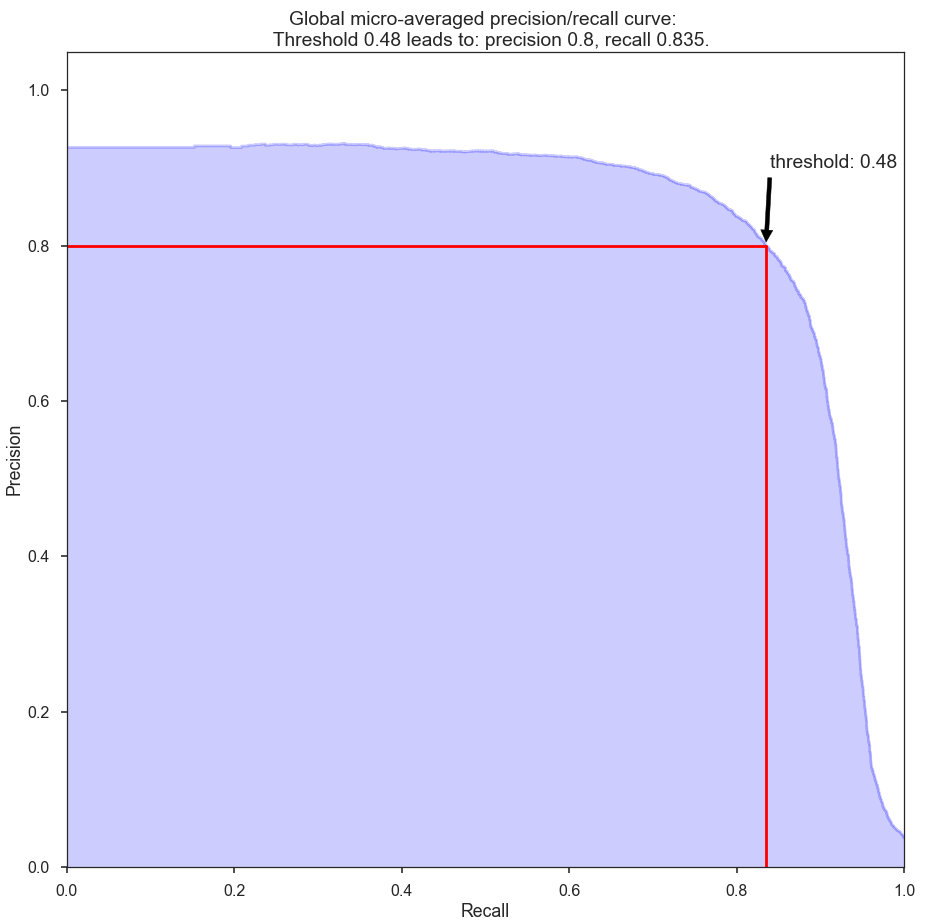
\includegraphics[scale=0.4]{./images/calibration/islabeledby_global_curve.png}
\caption{Global precision/recall curve for attribute 'product labels' (organic, made in France etc).}
\end{figure}

We can observe that if we apply a decision threshold of 0.48 on our prediction scores, we achieve:
\begin{itemize}
	\item a micro-average global precision of 0.80
	\item a micro-average global recall of 0.82
\end{itemize}

Given a decision threshold we will either favor recall or precision, each of them serves a different business objective:
\begin{itemize}
	\item favoring precision ensure that we don't make mistakes when pushing a suggestion to our users, it's a low-risk strategy, but with less impact
	\item favoring recall will ensure that we don't miss any suggestion that we could make on products (big impact), at the risk of being wrong sometimes.
\end{itemize}

The choice is a business choice, depending on what users favor. In our case, after some user interviews, it is clear that we prefer to favor precision. Users are frightened by wrong suggestions. Whereas the absence of suggestion has no negative impact.

\section{Missing labels}

\subsection{Strategies to handle incompletely labeled data}

Our data-quality challenge is quite paradoxical: \textbf{to increase data-quality, we have to rely on the data whose quality we want to improve.}

One issue is then than even if we manage to build a perfect classifier out of this invalid data, when we evaluate it, our precision will be low. Indeed imagine we have 200 products, 100 of them have in reality an 'Organic' label. 40 of them are actually labeled as such in our database (the other 60 being incompletely labeled). If our perfect classifier finds them all, the 100, our classifier precision will be around 40\% instead of 100\% because the test-set on which we will base our estimations will be biaised as well.

To overcome this challenge we adopted the following strategy:

\begin{itemize}
	\item make predictions based on available partially labeled data
	\item enrich our predictions with precision estimation based on each class precision given prediction score (see calibration part)
	\item bulk validate predictions which are not equal to products current attributes, based on:
	\begin{itemize}
		\item either textual search: our prediction are indexed in elasticsearch with product information allowing us to easily look for products whose description fields contain 'gluten'
		\item either categorical search: we know that all alcohols should have a 'pregnant warning pictogram'
		\item either by filtering predictions with the highest precision estimation
	\end{itemize}
	\item validated attributes predictions are stored in a database and override product attributes in classification workflow
\end{itemize}

In the following graphs, you can see that after a initial prediction of flavors attributes, we could detect with high degree a confidence some flavors attributes that were not labeled. After manually validating them, they were incorporated in the learning data-set and increased the training-support for each class. This improved data-quality led to a raise in flavors scores.

\begin{figure}[H]
\centering
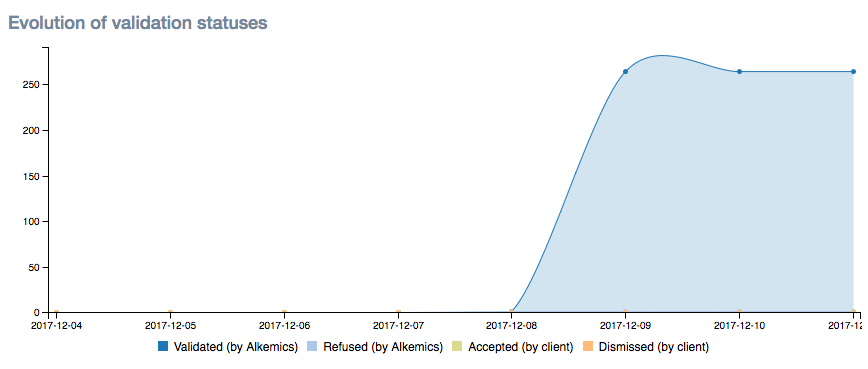
\includegraphics[scale=0.5]{./images/incompletely-labeled/validation-flavors.png}
\caption{Validated flavors predictions. On 2017-12-09, we validated about 250 predictions based on textual search.}
\end{figure}


\begin{figure}[H]
\centering
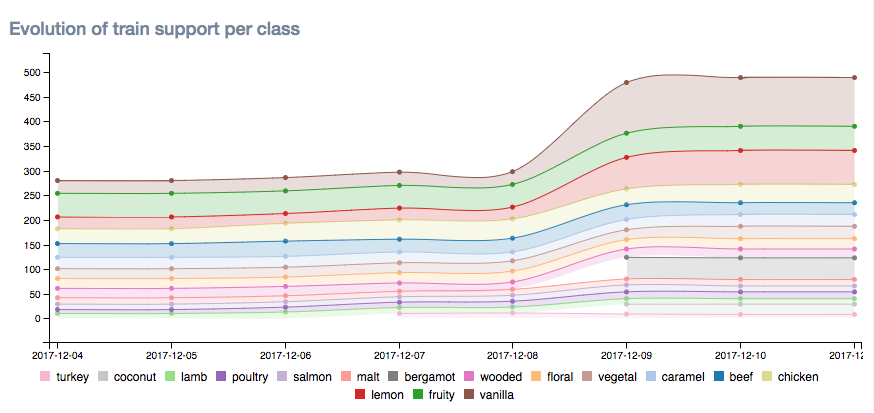
\includegraphics[scale=0.5]{./images/incompletely-labeled/train-support-flavors.png}
\caption{Train support for flavors classes increased as a consequence.}
\end{figure}


\begin{figure}[H]
\centering
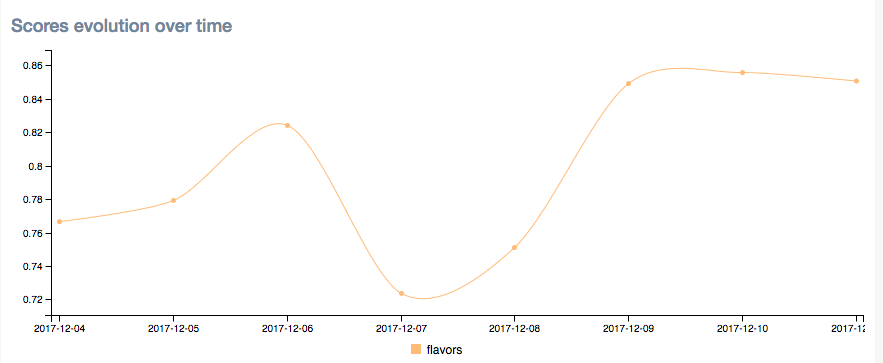
\includegraphics[scale=0.5]{./images/incompletely-labeled/scores-flavors.png}
\caption{Flavors scores are very volatile at the begining because of an insufficient number of training samples. After the validation on 2017-12-08, scores increased and score volatility decreased.}
\end{figure}


This process helps us increase the label density on some classes, which led to increased score.

When we use our predictions with best precision estimation to validate quickly, our process can be seen as a virtuous circle:
\begin{figure}[H]
\centering
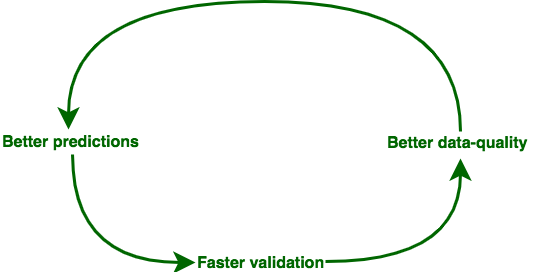
\includegraphics[scale=0.6]{./images/incompletely-labeled/virtuous-circle.png}
\caption{Virtuous validation workflow.}
\end{figure}

Inherently, when training a classifier to detect cases where our data is invalid on some samples, we generally put a stronger focus on precision rather than recall. Indeed:
\begin{itemize}
	\item in multilabel case, our invalid data is in nearly all cases missing values: which will lead to negatives instead of positives in our dataset.
	\item in case we predict a sample as positive for a given class, unfortunatly we will count it as a false positive instead of a true positive.
	\item thus it will impact recall, not precision.
\end{itemize}

\subsection{Iterative approach to bootstrap new classes}

It is sometimes necessary to adopt a pro-active approach on some classes with low scores or very low number of occurences. 
For instance, when we split a 'kind' (category) in multiple more detailed kinds.
After some iterations, there might be enough occurences to ensure sufficient scores.

\section{Evaluate results}

\subsection{Assess task difficulty}
Task difficulty can be assessed differently for each predicted field. It is dependent on multiple factors:
\begin{itemize}
	\item output size
	\begin{itemize}
		\item multiclass vs multilabel
		\item number of distinct classes
	\end{itemize}
	\item number of training samples
	\begin{itemize}
		\item dataset size
		\item classes and label densities: it will be difficult to predict labels that nearly never occur
	\end{itemize}
	\item is the information present in some form in features
\end{itemize}

\begin{tabularx}{\textwidth}{|l|r|X|X|X|X|X|X|r|}
\toprule
field & type &  label\ count & label\ cardinality &  label\ density &  label\ diversity &  nb\ classes &  nb\ samples & presence \\
\midrule
hazard			      &          multilabel &    2243     &     0.0408 &         0.0082 &             1090 &           5 &       54990 & very low\\
flavors               &          multilabel &    355      &     0.0065 &         0.0006 &              253 &          11 &       54990 & high \\
kind                  &          multiclass &    43335    &     1.0000 &         0.0057 &              175 &         175 &       43335 & low \\
ingredients			  &          multilabel &    54259    &     0.9867 &         0.0111 &            16810 &          89 &       54990 & high \\
labels 		          &          multilabel &    22803    &     0.4147 &         0.0078 &             7078 &          53 &       54990 & medium \\
\bottomrule
\end{tabularx}


\subsection{Assess how well our model perform}



\subsection{How much better can we do}




\section{To investigate further}

This section cover some topics we have not had time to cover for now, and that we think could help us deliver better results.

\subsection{Dive into kind tree-structure}
One of the attributes we predict has a tree structure: the 'kind', or product category. 

\begin{figure}[H]
\centering
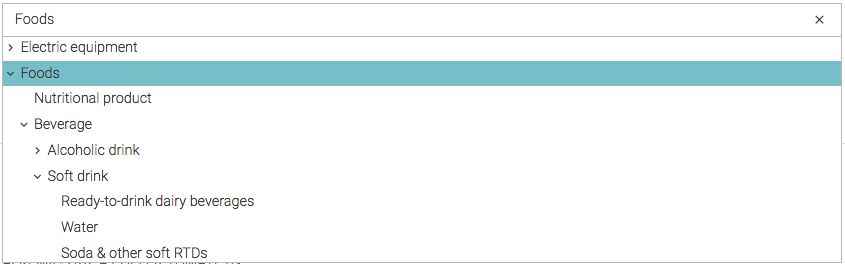
\includegraphics[scale=0.5]{./images/to-investigate/tree-structure.png}
\caption{Kind tree structure: Food contains Beverage, that contains Soft-dring, that contains Water, Soda etc..}
\end{figure}

We could take advantage of the information contained in the tree structure to improve classification. 

One possible strategy could be to create a kind similarity function, returning a scalar based on proximity in tree structure:
\begin{itemize}
	\item 'water' is very close to 'soft drink' because it is its direct child
	\item 'water' and 'bread' are very different because the shortest path between them is 4 edges.
\end{itemize}

This similarity function could be used as a coefficient in the cost function: 
\begin{itemize}
	\item if we predict 'soft drink' instead of 'water', the cost would be lowered because the error is minor
	\item if we predict 'bread' instead of 'water', the cost would be raised because the prediction is completely wrong
\end{itemize}

\subsection{Enforce better calibration / decision}
\subsection{Use images}
For now, use of google vision API to product text: labels, reading. This could be used in some neural networks embedding different types of objects.
\subsection{POS Tagging strategies to predict some fields}
Packaging, brand, etc..

\subsection{Tuning strategies}

For now: 

Quite random. Intuition. All dimensions except one or two. Difficult to understand.

\subsection{Higher order multilabel strategies}
Possible strategies include:
\begin{itemize}
	\item add layer to Fasttext neural network
	\item add independent layer, at the end: calibration (that will find correlation between classes)
\end{itemize}

Yet, these strategies are possible only with datasets with sufficient samples, otherwise we will overfit.

\subsection{Cross validation for sets with low label density}

\subsection{More workflow tests}

\cleardoublepage
\chapter*{Conclusion} % (fold)
\addcontentsline{toc}{chapter}{Conclusion}
\label{cha:conclusion}


During this project, we transformed a workflow dedicated to one multiclass field, to a much flexible and adaptable workflow.


Machine learning hype drives attention mostly to models and algorithms. 
Yet, this project convinced me that 90\% of a project success depends on pragmatism and implementation.

Fields to explore ....

Lot more to say when paper will be finished.

\chapter*{Acknowledgment}

Big up to @caillou for ML, and Alkemics as a whole for engineering skills.
Big up to MS BGD @Telecom for accepting me in 2017 promo

\addcontentsline{toc}{chapter}{Acknowledgment}

\cleardoublepage
\appendix
\chapter{Logistic Regression: from binary, to multiclass, to multilabel} % (fold)
\label{cha:multilabel_classification}


\section*{Common notations}


\subsection*{Notations for single-labeled samples}

\subsubsection*{Probabilistic notations}

\begin{outline}
\1 X random vector, $\mathcal{X} \subset \mathbb{R}^d$
\begin{align}
	X = \left[
	\begin{array}{cccc}
		X_{1} \\
		X_{2} \\
		\vdots\\
		X_{d} \\
	\end{array}\right]
\end{align}

\1 Y discrete random variable, $\mathcal{Y} $, with $|\mathcal{Y}|$ finite. In practice, Y is encoded as an integer, ie $\mathcal{Y} \subset \mathbb{N} $ and $Y \in \mathbb{N}$

\1 P joint probability of X and Y $(X,Y)$ (unknown).
\end{outline}

\subsubsection*{Empirical notations}

\begin{outline}
\1 $x$, a vector sample, which is a realization of X (the empirical counterpart of X) $x \in \mathbb{R}^d$:
\begin{align}
	x = \left[
	\begin{array}{cccc}
		x_{1} \\
		x_{2} \\
		\vdots\\
		x_{d} \\
	\end{array}\right]
\end{align}

\1 $y$, a sample, which is a realization of Y (the empirical counterpart of Y): $y \in \mathcal{Y} \subset \mathbb{N}$

\1 $ \mathcal{D}_m = \{(x^{(i)}, y^{(i)}), i \in 1,m\} \in (\mathcal{X},\mathcal{Y})^m$ a learning set containing $m$ samples $iid$ and from P.\\
\end{outline}

Note:
For the $i^{th}$ sample, $x^{(i)}$ $y^{(i)}$, which are vectors, we'll respectively denote the $j^{th}$ component as follow: $x_j^{(i)}$ and $y_j^{(i)}$


\subsection*{Notations for multi-labeled samples}

Everything is the same except that labels are no longer scalars but vectors, with $K = |\mathcal{Y}|$:

\begin{outline}
\1 Y random vector, $\mathcal{Y} \subset \mathbb{N}^d$
\begin{align}
	Y = \left[
	\begin{array}{cccc}
		Y_{1} \\
		Y_{2} \\
		\vdots\\
		Y_{K} \\
	\end{array}\right]
\end{align}

\1 Y discrete random variable, $\mathcal{Y} $, with $|\mathcal{Y}|$ finite. In practice, Y is encoded as an integer, ie $\mathcal{Y} \subset \mathbb{N} $ and $Y \in \mathbb{N}$

\1 P joint probability of X and Y $(X,Y)$ (unknown).
\end{outline}






\section{Binary case: Logistic regression} % (fold)
\label{sec:workflow}


We want to predict the value of $y^{(i)}$ for the example $x^{(i)}$ using a function $y = h_\theta(x) $ with binary-valued labels $\left(y^{(i)} \in \{0,1\}\right)$. We want to predict the probability that a given example belongs to the “1” class versus the probability that it belongs to the “0” class. Specifically, we will try to learn a function of the form:

\subsection{Model}
\begin{align}
	P(Y=1|X=x) &= f_\theta(x) \\
			   &= \frac{1}{1 + \exp(-\theta^\top x)} \\
			   &= \sigma(\theta^\top x),\\
	P(Y=0|X=x) &= 1 - f_\theta(x) \\
			   &= \sigma(-\theta^\top x)
\end{align}

With:
\begin{align}
	\sigma(z) \equiv \frac{1}{1 + \exp(-z)}
\end{align}

the “logistic” function. It is an S-shaped function that “squashes” the value of $\theta^\top x$ into the range [0, 1] so that we may interpret $f_\theta(x)$ as a probability. 

Our goal is to search for a value of $\theta$ so that the probability $P(Y=1|x) = f_\theta(x)$ is large when x belongs to the “1” class and small when x belongs to the “0” class (so that $P(Y=0|x)$ is large). 

For further use, note than for $k \in \{0,1\}$:
\begin{align}
	P(Y=k|x) = (f_\theta(x))^k \times (1 - f_\theta(x))^{(1-k)}
\end{align}

\subsection{Objective}
For a set of training examples with binary labels $\{ (x^{(i)}, y^{(i)}) : i=1,\ldots,m\}$, assuming that the $m$ training examples were generated independently, we can then write down the likelihood of the parameters as:
\begin{align}
	L(\theta) &= \prod_{i=1}^m P(Y=y^{(i)} | x^{(i)}, \theta) \\
			  &= \prod_{i=1}^m (f_\theta(x^{(i)}))^{y^{(i)}} \times (1 - f_\theta(x^{(i)})^{(1-y^{(i)})})
\end{align}

It will be easier to maximize the log likelihood:
\begin{align}
	l(\theta) &= \log L(\theta) \\
			  &= \log \left( \prod_{i=1}^m P(Y=y^{(i)} | x^{(i)}) \right) \\
			  &= \sum_{i=1}^m \left( y^{(i)}\log f_\theta(x^{(i)}) + (1-y^{(i)})\log (1 - f_\theta(x^{(i)})) \right)
\end{align}

It is the same as minimizing the following (cross entropy loss):
\begin{align}
	E(\theta) = - \sum_i \left(y^{(i)} \log( f_\theta(x^{(i)}) ) + (1 - y^{(i)}) \log( 1 - f_\theta(x^{(i)}) ) \right).
\end{align}


Note that only one of the two terms in the summation is non-zero for each training example (depending on whether the label $y^{(i)}$ is 0 or 1). When $y^{(i)} = 1$ minimizing the cost function means we need to make $f_\theta(x^{(i)})$ large, and when $y^{(i)} = 0$ we want to make $1 - f_\theta$ large as explained above.

We now have a cost function that measures how well a given hypothesis $f_\theta$ fits our training data. We can learn to classify our training data by minimizing $E(\theta)$ to find the best choice of $\theta$. Once we have done so, we can classify a new test point as “1” or “0” by checking which of these two class labels is most probable: if $P(y=1|x) > P(y=0|x)$ then we label the example as a “1”, and “0” otherwise. This is the same as checking whether $f_\theta(x) > 0.5$.

\subsection{Optimization}
We want to minimize $E(\theta)$. The derivative of $E(\theta)$ as given above with respect to $\theta_j$ is:

\begin{align}
	\frac{\partial E(\theta)}{\partial \theta_j} = \sum_i x^{(i)}_j (f_\theta(x^{(i)}) - y^{(i)})
\end{align}

Demonstration available \href{https://math.stackexchange.com/questions/477207/derivative-of-cost-function-for-logistic-regression}{here}.

Written in its vector form, the entire gradient can be expressed as ($x^{(i)}$ being a d dimensional vector, with d being the dimension of each sample feature):

\begin{align}
	\nabla_\theta E(\theta) 
	&= 
	\begin{bmatrix}
		\frac{\partial E(\theta)}{\partial \theta_1}\\
		\frac{\partial E(\theta)}{\partial \theta_2}\\
		\vdots\\
		\frac{\partial E(\theta)}{\partial \theta_d}
	\end{bmatrix}
	=
		\sum_i x^{(i)} (f_\theta(x^{(i)}) - y^{(i)})
\end{align}

We can then apply gradient descent to find global minimum since $E(\theta)$ is convex, with learning rate $\alpha$:

\begin{align}
	\theta \leftarrow \theta - \alpha \nabla_\theta E(\theta)
\end{align}

\subsection{Vectorial representations}
\begin{align}
	\theta = \left[
	\begin{array}{cccc}
		\theta_{1} \\
		\theta_{2} \\
		\vdots\\
		\theta_{d} \\
	\end{array}\right]
\end{align}

\begin{align}
	\mathcal{D}_m = 
	\left[
		\begin{array}{cccc}
			- x^{(1)} - \\
			- x^{(2)} -  \\ 
			\vdots \\
			- x^{(m) - } 
		\end{array}
	\right]
\end{align}








\section{Multiclass case: Softmax regression}


Softmax regression (or multinomial logistic regression) is a generalization of logistic regression to the case where we want to handle multiple classes. In logistic regression we assumed that the labels were binary: $y^{(i)} \in \{0,1\}$. Softmax regression allows us to handle $ y^{(i)} \in \{1,\ldots,K\}$ where K is the number of classes.

In the softmax regression setting, we are interested in multi-class classification (as opposed to only binary classification), and so the label y can take on K different values, rather than only two. Thus, in our training set $\{ (x^{(1)}, y^{(1)}), \ldots, (x^{(m)}, y^{(m)}) \}$, we now have that $y^{(i)} \in \{1, 2, \ldots, K\}$. (Note that our convention will be to index the classes starting from 1, rather than from 0.) 

\subsection{Model}

Given a test input x, we want our hypothesis to estimate the probability $P(Y=k | x)$ for each value of $k = 1, \ldots,$ K. i.e. we want to estimate the class probabilities of the K different possible labels. Thus, our hypothesis function will output multinomial distribution: a K-dimensional vector (whose elements sum to 1) giving us our K estimated probabilities. Concretely, our hypothesis $f_{\theta}(x)$ takes the form:

\begin{align}
	f_\theta(x)
	=
	\begin{bmatrix}
		P(Y = 1 | x; \theta) \\ P(Y = 2 | x; \theta) \\ \vdots \\ P(Y = K | x; \theta) 
	\end{bmatrix} 
	= 
	\frac{1}{ \sum_{j=1}^{K}{\exp(\theta^{(j)\top} x) }} 
	\begin{bmatrix} 
		\exp(\theta^{(1)\top} x ) \\ \exp(\theta^{(2)\top} x ) \\ \vdots \\ \exp(\theta^{(K)\top} x ) \\ 
	\end{bmatrix} 
\end{align}

Here $\theta^{(1)}, \theta^{(2)}, \ldots, \theta^{(K)} \in \mathbb{R}^{d}$ are the parameters of our model. Notice that the term $\frac{1}{ \sum_{j=1}^{K}{\exp(\theta^{(j)\top} x) } }$ normalizes the distribution, so that it sums to one.

For convenience, we will also write $\theta$ to denote all the parameters of our model. When you implement softmax regression, it is usually convenient to represent $\theta$ as a n-by-K matrix obtained by concatenating $\theta^{(1)}, \theta^{(2)}, \ldots, \theta^{(K)}$ into columns, so that:

\begin{align}
	\theta = \left[\begin{array}{cccc}| & | & | & | \\ \theta^{(1)} & \theta^{(2)} & \cdots & \theta^{(K)} \\ | & | & | & | \end{array}\right]
\end{align}

With each $\theta^{(i)}$ being a vector $\in \mathbb{R}^{d}$:

\begin{align}
	\theta^{(i)} = \left[
		\begin{array}{cccc}
			\theta_{1}^{(i)} \\
			\theta_{2}^{(i)} \\
			\vdots \\
			\theta_{d}^{(i)}
		\end{array}\right]
\end{align}


\subsection{Objective}

We now describe the cost function that we’ll use for softmax regression.

For a set of training examples with multiclass labels $\{ (x^{(i)}, y^{(i)}) : i=1,\ldots,m\}$, assuming that the $m$ training examples were generated independently, we can then write down the likelihood of the parameters as:
\begin{align}
	L(\theta) &= \prod_{i=1}^m P(Y=y^{(i)} | x^{(i)} ) \\
			  &= \prod_{i=1}^m (f_\theta(x^{(i)}))^{y^{(i)}} \times (1 - f_\theta(x^{(i)})^{(1-y^{(i)})})
\end{align}

It will be easier to maximize the log likelihood:
\begin{align}
	l(\theta) &= \log L(\theta) \\
			  &= \log \left( \prod_{i=1}^m P(Y=y^{(i)} | x^{(i)}) \right) \\
			  &= \sum_{i=1}^m \left( y^{(i)}\log f_\theta(x^{(i)}) + (1-y^{(i)})\log (1 - f_\theta(x^{(i)})) \right)
\end{align}

It is the same as minimizing the following (cross entropy loss):

\begin{align} 
	E(\theta) = - \left[ \sum_{i=1}^{m} \sum_{k=1}^{K} \mathds{1}\left\{y^{(i)} = k\right\} \log \frac{\exp(\theta^{(k)\top} x^{(i)})}{\sum_{j=1}^K \exp(\theta^{(j)\top} x^{(i)})}\right] 
\end{align}

Notice that this generalizes the logistic regression cost function, which could also have been written:

\begin{align}
	E(\theta) &= - \left[ \sum_{i=1}^m (1-y^{(i)}) \log (1-f_\theta(x^{(i)})) + y^{(i)} \log f_\theta(x^{(i)}) \right] \\ 
			  &= - \left[ \sum_{i=1}^{m} \sum_{k=0}^{1} \mathds{1}\left\{y^{(i)} = k\right\} \log P(y^{(i)} = k | x^{(i)} ; \theta) \right] 
\end{align}
The softmax cost function is similar, except that we now sum over the K different possible values of the class label. Note also that in softmax regression, we have that

\begin{align}
	P(y^{(i)} = k | x^{(i)} ; \theta) = \frac{\exp(\theta^{(k)\top} x^{(i)})}{\sum_{j=1}^K \exp(\theta^{(j)\top} x^{(i)}) }
\end{align}

\subsection{Optimization}

We cannot solve for the minimum of $E(\theta)$ analytically, and thus as usual we’ll resort to an iterative optimization algorithm. Taking derivatives, one can show that the gradient is:

\begin{align} \nabla_{\theta^{(k)}} E(\theta) = - \sum_{i=1}^{m}{ \left[ x^{(i)} \left( \mathds{1} \{ y^{(i)} = k\} - P(Y^{(i)} = k | x^{(i)}; \theta) \right) \right] } \end{align}

In particular, $\nabla_{\theta^{(k)}} E(\theta)$ is itself a vector, so that its j-th element is $\frac{\partial E(\theta)}{\partial \theta_{lk}}$ the partial derivative of $E(\theta)$ with respect to the j-th element of $\theta^{(k)}$.

Armed with this formula for the derivative, one can then plug it into a standard optimization package and have it minimize $E(\theta)$.

\subsection{Properties of softmax regression parameterization}

Softmax regression has an unusual property that it has a “redundant” set of parameters. To explain what this means, suppose we take each of our parameter vectors $\theta^{(j)}$, and subtract some fixed vector $\psi$ from it, so that every $\theta^{(j)}$ is now replaced with $\theta^{(j)} - \psi$ (for every j=1, $\ldots$, k). Our hypothesis now estimates the class label probabilities as

\begin{align} 
P(y^{(i)} = k | x^{(i)} ; \theta) &= \frac{\exp((\theta^{(k)}-\psi)^\top x^{(i)})}{\sum_{j=1}^K \exp( (\theta^{(j)}-\psi)^\top x^{(i)})} \\ &= \frac{\exp(\theta^{(k)\top} x^{(i)}) \exp(-\psi^\top x^{(i)})}{\sum_{j=1}^K \exp(\theta^{(j)\top} x^{(i)}) \exp(-\psi^\top x^{(i)})} \\ &= \frac{\exp(\theta^{(k)\top} x^{(i)})}{\sum_{j=1}^K \exp(\theta^{(j)\top} x^{(i)})}. 
\end{align}
In other words, subtracting $\psi$ from every $\theta^{(j)}$ does not affect our hypothesis’ predictions at all! This shows that softmax regression’s parameters are “redundant.” More formally, we say that our softmax model is ”‘overparameterized,”’ meaning that for any hypothesis we might fit to the data, there are multiple parameter settings that give rise to exactly the same hypothesis function $h_\theta$ mapping from inputs x to the predictions.

Further, if the cost function $E(\theta)$ is minimized by some setting of the parameters $(\theta^{(1)}, \theta^{(2)},\ldots, \theta^{(k)})$, then it is also minimized by $(\theta^{(1)} - \psi, \theta^{(2)} - \psi,\ldots, \theta^{(k)} - \psi)$ for any value of $\psi$. Thus, the minimizer of $E(\theta)$ is not unique. (Interestingly, $E(\theta)$ is still convex, and thus gradient descent will not run into local optima problems. But the Hessian is singular/non-invertible, which causes a straightforward implementation of Newton’s method to run into numerical problems.)

Notice also that by setting $\psi = \theta^{(K)}$, one can always replace $\theta^{(K)}$ with $\theta^{(K)} - \psi = \vec{0}$ (the vector of all 0’s), without affecting the hypothesis. Thus, one could “eliminate” the vector of parameters $\theta^{(K)}$ (or any other $\theta^{(k)}$, for any single value of k), without harming the representational power of our hypothesis. Indeed, rather than optimizing over the $K\cdot$ n parameters $(\theta^{(1)}, \theta^{(2)},\ldots, \theta^{(K)}) (where \theta^{(k)} \in \Re^{n})$, one can instead set $\theta^{(K)} = \vec{0}$ and optimize only with respect to the $K \cdot$ n remaining parameters.

\subsection{Relationship to Logistic Regression}

In the special case where K = 2, one can show that softmax regression reduces to logistic regression. This shows that softmax regression is a generalization of logistic regression. Concretely, when K=2, the softmax regression hypothesis outputs

\begin{align} 
	f_\theta(x) &= \frac{1}{ \exp(\theta^{(1)\top}x) + \exp( \theta^{(2)\top} x^{(i)} ) } \begin{bmatrix} \exp( \theta^{(1)\top} x ) \\ \exp( \theta^{(2)\top} x ) \end{bmatrix} 
\end{align}
Taking advantage of the fact that this hypothesis is overparameterized and setting $\psi = \theta^{(2)}$, we can subtract $\theta^{(2)}$ from each of the two parameters, giving us

\begin{align} f(x) &= \frac{1}{ \exp( (\theta^{(1)}-\theta^{(2)})^\top x^{(i)} ) + \exp(\vec{0}^\top x) } \begin{bmatrix} \exp( (\theta^{(1)}-\theta^{(2)})^\top x ) \exp( \vec{0}^\top x ) \\ \end{bmatrix} \\ &= \begin{bmatrix} \frac{1}{ 1 + \exp( (\theta^{(1)}-\theta^{(2)})^\top x^{(i)} ) } \\ \frac{\exp( (\theta^{(1)}-\theta^{(2)})^\top x )}{ 1 + \exp( (\theta^{(1)}-\theta^{(2)})^\top x^{(i)} ) } \end{bmatrix} \\ &= \begin{bmatrix} \frac{1}{ 1 + \exp( (\theta^{(1)}-\theta^{(2)})^\top x^{(i)} ) } \\ 1 - \frac{1}{ 1 + \exp( (\theta^{(1)}-\theta^{(2)})^\top x^{(i)} ) } \\ \end{bmatrix} 
\end{align}
Thus, replacing $\theta^{(2)}-\theta^{(1)}$ with a single parameter vector $\theta'$, we find that softmax regression predicts the probability of one of the classes as $\frac{1}{ 1 + \exp(- (\theta')^\top x^{(i)} ) }$, and that of the other class as $1 - \frac{1}{ 1 + \exp(- (\theta')^\top x^{(i)} ) }$, same as logistic regression.



\subsection{Vectorial representations}
\begin{align}
	\theta = \left[\begin{array}{cccc}| & | & | & | \\ \theta^{(1)} & \theta^{(2)} & \cdots & \theta^{(K)} \\ | & | & | & | \end{array}\right]
\end{align}












\section{Multilabel case: 'multi-binary' regression}

In this case, suppose you want to predict which pictograms are present on a product, like 'organic food', 'product of the year' or 'made in France'. Each product can have multiple labels.

One possibility is to treat each class as an independent binary problem. Our sample label is no longer a scalar, but a vector of $d$ dimensions (number of possible classes).

\begin{align}
	Y = \left[
	\begin{array}{cccc}
		Y_{1} \\
		Y_{2} \\
		\vdots\\
		Y_{K} \\
	\end{array}\right]
\end{align}

With $Y_{i} \in \{0, 1\}$

Our sample then is not a single value but an indicator vector:

\begin{align}
	y = \left[
	\begin{array}{cccc}
		y_{1} \\
		y_{2} \\
		\vdots\\
		y_{K} \\
	\end{array}\right]
\end{align}

With $y_{i} \in \{0, 1\}$

\begin{align}
y_{i} = \left\{
    \begin{array}{ll}
        1 & \mbox{if the } i^{th} \mbox{ class is positive} \\
        0 & \mbox{else.}
    \end{array}
\right.
\end{align}

\subsection{Model}

Given a test input x, we want our hypothesis to independently estimate the probability that $P(Y=y | x)$. More specifically, for each possible class, we want to estimate the probability that the class is positive. Thus, our hypothesis will output a K-dimensional vector (whose elements don't sum to 1! in opposition to softmax regression) giving us our K estimated probabilities. Concretely, our model $F_{\theta}(x)$ takes the form:

\begin{align}
	F_\theta(x) 
		&= \begin{bmatrix} 
			f_{\theta^{(1)}}(x) \\ 
			f_{\theta^{(2)}}(x) \\ 
			\vdots \\ 
			f_{\theta^{(K)}}(x) 
		\end{bmatrix} \\
	\theta &= \left[\begin{array}{cccc}| & | & | & | \\ \theta^{(1)} & \theta^{(2)} & \cdots & \theta^{(K)} \\ | & | & | & | \end{array}\right]
\end{align}


With each $\theta^{(i)}$ being a vector $\in \mathbb{R}^{d}$.
For $i \in [1, K]$:

\begin{align}
	\theta^{(i)} = \left[
		\begin{array}{cccc}
			\theta_{1}^{(i)} \\
			\theta_{2}^{(i)} \\
			\vdots \\
			\theta_{d}^{(i)}
		\end{array}\right]
\end{align}


\begin{align}
	f_{\theta^{(i)}}(x) 
	&= P(Y_i = 1 | x; \theta^{(i)}(x)) \\
	&= \frac{1}{1 + \exp(-\theta^{(i)\top} x)}\\
	&= \sigma(\theta^{(i)\top} x)
\end{align}




\subsection{Objective}


For a set of training examples with multilabel samples $\{ (x^{(i)}, y^{(i)}) : i=1,\ldots,m\}$, assuming that the $m$ training examples were generated independently, we can then write down the likelihood of the parameters as:
\begin{align}
	L(\theta) &= \prod_{i=1}^m P(Y=y^{(i)} | x^{(i)} ) \\
\end{align}

Making the assumptions that all classes are independent (which is in pratice usually inaccurate but theorically necessary):

\begin{align}
	L(\theta) &= \prod_{i=1}^m \prod_{j=1}^K P(Y_j=y_j^{(i)} | x^{(i)}) 
\end{align}


It will be easier to minimize the negative log likelihood:
\begin{align}
	E(\theta) &=  - \log L(\theta) \\
			  &= - \sum_{i=1}^m \sum_{j=1}^K \log  P(Y_j=y_j^{(i)} | x^{(i)}) \\
  			  &= -  \sum_{i=1}^m \sum_{j=1}^K
  			  	\left\{
				    \begin{array}{ll}
				        \log (\sigma(\theta^{(j)\top} x^{(i)})) & \mbox{if } y_j^{(i)} =1 \\
				        \log (1 - \sigma(\theta^{(j)\top} x^{(i)})) & \mbox{if } y_j^{(i)} =0 
				    \end{array}
				\right. \\
\end{align}


\subsection*{Optimization}

We want to minimize $E(\theta)$. The derivative of $E(\theta)$ as given above with respect to $\theta_j^{(k)}$, $j \in [1,d]$ is:

\begin{align}
	\frac{\partial E(\theta)}{\partial \theta_k^{(j)}} 
	&= \sum_{i=1}^m x^{(i)}_k (\sigma(\theta^{(j)\top} x^{(i)}) - y_j^{(i)}) \\
	&= \sum_{i=1}^m x^{(i)}_k (f_{\theta^{(j)}}(x^{(i)})  - y_j^{(i)}) 
\end{align}

Hints:
\begin{align}
	\frac{\partial (\theta^{(j)\top} x^{(i)}) }{\partial \theta_k^{(j)}}  &= x_k^{(i)} 
\end{align}
\begin{align}
	(log \circ \sigma)'(t) &= \sigma(-t)
\end{align}


The entire gradient can be expressed as a $d \times K$ dimensional matrix (with d being the dimension of each sample feature and K the number of classes):

\begin{align}
	\nabla_\theta E(\theta) 
	&= 
	\begin{bmatrix}
		\frac{\partial E(\theta)}{\partial \theta_1^{(1)}} 	& \dots 						& \frac{\partial E(\theta)}{\partial \theta_1^{(K)}} \\
		\dots 												&  \frac{\partial E(\theta)}{\partial \theta_i^{(j)}} 	& \dots \\
		\frac{\partial E(\theta)}{\partial \theta_d^{(1)}} 	& \dots 						& \frac{\partial E(\theta)}{\partial \theta_d^{(K)}}
	\end{bmatrix} 
\end{align}

We can then apply gradient descent to find global minimum since $E(\theta)$ is convex, with learning rate $\alpha$:

\begin{align}
	\theta \leftarrow \theta - \alpha \nabla_\theta E(\theta)
\end{align}



\subsection*{Context}

This method is nearly equivalent to applying binary relevance (problem transformation method) to logistic regression.

Yet:
\begin{outline}
\1 it can be considered as an adaptative method (in opposition to problem transformation method): the algorithm is adapted to fit the data
\1 an advantage of this algorithm is to be able to compute gradient for each sample evaluated during training. This allows to retropropagate gradient to previous layers in the context of a multi-layer neural network. In comparison, using binary relevance method with any classifier does not allow this.
\end{outline}



\pagebreak

\subsection*{Gradient retro-propagation in multilayer neural network}

\subsubsection*{Network definition}

Suppose a previous layer $h$ (taking a vector x of given size in ouput space of size d) as follow:
\begin{align}
	h = 
	\begin{bmatrix} 
		h_1 \\
		h_2 \\
		\vdots \\
		h_d
	\end{bmatrix}
\end{align}


With $g$ being a function parametrized by w so that:
\begin{align}
	h_j = g_{W^{(j)}}(x)
\end{align}
With $W$ being the matrix of weights from input to hidden layer.


Let's denote:

\begin{align}
	s_k  = \theta^{(k)\top} h = \sum_{j=1}^{d} \theta^{(k)\top}_j h_j 
\end{align}

we can express $f$ as, $\forall k \in [1, K]$:

\begin{align}
	f_k  = \sigma(s_k) = \sigma( \sum_{j=1}^{d} \theta^{(k)\top}_j h_j) 
\end{align}

Lets consider the following error on one sample $(x, y)$:

\begin{align}
	E = - \sum_{k=1}^K
  			  	\left\{
				    \begin{array}{ll}
				        \log (f_k) & \mbox{if } y_k =1 \\
				        \log (1 - f_k) & \mbox{if } y_k =0
				    \end{array}
				\right.
\end{align}

This error is relevant since the minimization of this error is equivalent to maximizing the maximum of (log-)likelihood.
Plus, it is interpretable: if the $k^{th}$ component $y_k$ is:
\begin{itemize}
	\item positive ($y_k=1$): then the loss increase if $f_k$ is near 0, and decrease if $f_k$ is near 1.
	\item negative ($y_k=0$): then the loss decrease if $f_k$ is near 0, and increase if $f_k$ is near 1.
\end{itemize}



We can represent it as the following multilayer network:

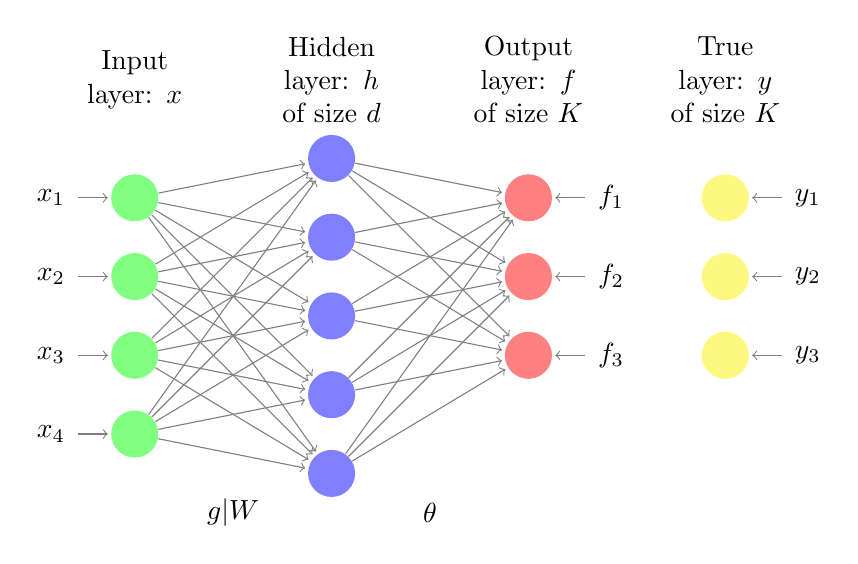
\begin{tikzpicture}[shorten >=1pt,->,draw=black!50, node distance=\layersep]
    \tikzstyle{every pin edge}=[<-,shorten <=1pt]
    \tikzstyle{neuron}=[circle,fill=black!25,minimum size=17pt,inner sep=0pt]
    \tikzstyle{input neuron}=[neuron, fill=green!50];
    \tikzstyle{output neuron}=[neuron, fill=red!50];
    \tikzstyle{hidden neuron}=[neuron, fill=blue!50];
    \tikzstyle{true neuron}=[neuron, fill=yellow!50];
    \tikzstyle{annot} = [text width=4em, text centered]

    % Draw the input layer nodes
    \foreach \name / \y in {1,...,4}
    % This is the same as writing \foreach \name / \y in {1/1,2/2,3/3,4/4}
        \node[input neuron, pin=left:$x_{\y}$ ] (I-\name) at (0,-\y) {};

    % Draw the hidden layer nodes
    \foreach \name / \y in {1,...,5}
        \path[yshift=0.5cm] node[hidden neuron] (H-\name) at (\layersep,-\y cm) {};

    % Draw the output layer node
    % \node[output neuron,pin={[pin edge={->}]right:Output}, right of=H-3] (O) {};

	\foreach \name / \y in {1,...,3}
        \node[output neuron, pin=right:$f_{\y}$ ] (O-\name) at (\layersep*2,-\y) {};

    % Draw the true layer node

	\foreach \name / \y in {1,...,3}
        \node[true neuron, pin=right:$y_{\y}$ ] (T-\name) at (\layersep*3,-\y) {};


    % Connect every node in the input layer with every node in the
    % hidden layer.
    \foreach \source in {1,...,4}
        \foreach \dest in {1,...,5}
            \path (I-\source) edge (H-\dest);

    % Connect every node in the hidden layer with the output layer
    \foreach \source in {1,...,5}
        \foreach \dest in {1,...,3}
	        \path (H-\source) edge (O-\dest);

    % Annotate the layers
    \node[annot,above of=H-1, node distance=1cm] (hl) {Hidden layer: $h$ of size $d$};
    \node[annot,left of=hl] {Input layer: $x$};
    \node[annot,right of=hl] (ol) {Output layer: $f$ of size $K$};
    \node[annot,right of=ol] {True layer: $y$ of size $K$};

    \node[annot] (W) at (\layersep/2,-5) {$g|W$};
    \node[annot] (W) at (\layersep*3/2,-5) {$\theta$};

\end{tikzpicture}

\subsubsection*{Gradient retropropagation}


\begin{align}
	\frac{ \partial E } { \partial f_k } = 
		\left\{
		    \begin{array}{ll}
		        - \frac{1}{f_k} & \mbox{if } y_k =1 \\
		        \frac{1}{1 - f_k} & \mbox{if } y_k =0
		    \end{array}
		\right.
\end{align}


\begin{align}
	\frac{ \partial E } { \partial s_k } 
		=  
		\frac{ \partial E } { \partial f_k } \cdot \frac{ \partial f_k } { \partial s_k } 
		&=
		\left\{
		    \begin{array}{ll}
		        - \frac{1}{f_k} \cdot f_k (1 - f_k)& \mbox{if } y_k =1 \\
		        \frac{1}{1 - f_k} \cdot f_k (1 - f_k)& \mbox{if } y_k =0
		    \end{array}
		\right. \\
		&=
		\left\{
		    \begin{array}{ll}
		       f_k - 1 & \mbox{if } y_k =1 \\
		       f_k & \mbox{if } y_k =0
		    \end{array}
		\right. \\
		&= f_k - y_k
\end{align}



\begin{align}
	\frac{\partial E}{\partial \theta_i^{(k)}} 
	= 
	\frac{\partial E}{\partial s_k} \cdot \frac{\partial s_k}{\partial \theta_i^{(k)}} 
	= 
	h_i (f_k - y_k)
\end{align}


Trick: derivate $E$ in regard to $s_k$:
\begin{align}
	\frac{\partial E}{\partial h_i} 
	&= 
	\sum_{k=1}^K \frac{\partial E}{\partial s_k} \cdot \frac{\partial s_k}{\partial h_i} \\
	&= 
	\sum_{k=1}^K \theta_i^{(k)} (f_k - y_k)
\end{align}

We now have the gradient of E in regard to the output of the hidden layer. The equation to update $W$ will depend of which $g$ is chosen.

\cleardoublepage

\bibliographystyle{plain}
\bibliography{biblio}

\end{document}
